%===============================================================

%Template for UPC-TALP based on CTU and modified to match UPC-TALP colors and style
%The original template from Czech Technical University  % Author: Martin Malý.
% They are defined by new graphical manual - 2017.
% Share and modify as you like. Keep the name of the authors.
% It is forbidden to use the template commercially.
%===============================================================

%\documentclass[aspectratio=169]{beamer}
\documentclass[]{beamer}

\input{preamble.tex}

%====================================================
%========== DEFINITION OF AUTHORS ETC...=============
%====================================================
\author[TARAN Seminar]{LEDOUX Louis}
\institute[]{Universitat Politècnica de Catalunya (UPC)\\ Barcelona Supercomputing Center (BSC)
\vspace{2mm} \\
%Advisors:  \\ Dr. Marc Casas \\ Dr. Eduard Ayguad\'e
%\vspace{2mm}
}
\title[]{The Walls and the Dark Silicon Era: An Arithmetic Perspective}


%\date[\today]{\small{Thesis Defense} \\ \small{\today}}
\date[December 2nd, 2024]{\small{TARAN Seminar} \\ \small{December 2nd, 2024}}

%====================================================
%========== BEGINNING OF DOCUMENT ===================
%====================================================


\begin{document}


\begin{frame}[plain]
	\titlepage
	\begin{center}%
		\vspace{-0.2cm}
		\includegraphics[height=1cm]{./figs/darkblue-logo.pdf}
		\hspace{2mm}
		\includegraphics[height=1cm]{./figs/bsc_logo_2.jpg}
	\end{center}
\end{frame}

\begin{frame}
\frametitle{Agenda}
	\begin{enumerate}
		\item \textit{Marenotrum et ego}
		\item Presentation context
		\item Tradeoff 1: Accuracy vs. Energy Efficiency
		\item Tradeoff 2: Latency vs. Parallelism
		\item Closing
	\end{enumerate}
\end{frame}

\section{Marenostrum et ego}
\graphicspath{{./figs/}}
\subsection{Ego}

\begin{frame}
	\frametitle{Who Am I? — Basic Info}
	\begin{columns}
	\begin{column}{0.65\textwidth}
		\begin{itemize}
			\item Louis Ledoux, 29 yo, PhD arithmetic HW
			\item My website, a pointer to many things:
			\begin{itemize}
				\item papers
				\item CV
				\item projects
				\item this presentation's slides
			\end{itemize}
		\end{itemize}
	\end{column}
	\begin{column}{0.35\textwidth}
		\begin{figure}[H]
			\centering
			\includegraphics[width=\textwidth]{QR-Mysite.png}
			\caption{https://bynaryman.github.io/}
			\label{fig:qr_website}
		\end{figure}
	\end{column}
	\end{columns}
\end{frame}

\begin{frame}
	\frametitle{Who Am I? — Research Interests}
	\begin{itemize}
		\item<1-> \textbf{Computer Architecture:}
		\begin{itemize}
			\item Floating-Point Units, Systolic Arrays, Matrix-Matrix Multiply (MMM) Units
			\item GPUs, FPGAs, workload-specific accelerators
		\end{itemize}
		\item<2-> \textbf{Computer Arithmetic:}
		\begin{itemize}
			\item Number Representations, Posit, IEEE 754 Standards
			\item FloPoCo, Application-Specific Circuits
			\item Kulisch Accumulator
		\end{itemize}
		\item<3-> \textbf{High Performance Computing:}
		\begin{itemize}
			\item BLAS, GEMMs, Heterogeneous Workloads
			\item Numerical Analysis, Supercomputing
		\end{itemize}
	\end{itemize}
\end{frame}

\begin{frame}
	\frametitle{Who Am I? — Education}
	\begin{itemize}
		\item<1-> \textbf{2013-2015} - Integrated Preparatory Class (CUPGE) - \textit{Rennes}
		\item<2-> \textbf{2015-2018} - ESIR (\'Ecole Supérieur d'Ing\'enieurs de \textit{Rennes})
		\begin{itemize}
			\item Engineer + Master's Degree, specializing in Computer Science.
			\item Last year coopt student at b<>com made me go to hardware
		\end{itemize}
		\item<3-> \textbf{2018-2024} - UPC (Universitat Politècnica de Catalunya) - \textit{Barcelona}
		\begin{itemize}
			\item Also Barcelona Supercomputing Center (BSC) / Marenostrum4/5
			\item Thesis: \textit{``Floating-Point Arithmetic Paradigms for High-Performance Computing: Software Algorithms and Hardware Designs''}
		\end{itemize}
		\item<4-> \textbf{2025-2027} - Coming Soon: Postdoc at INSA - \textit{Lyon}
		\begin{itemize}
			\item with Florent de Dinechin on MLIR-FloPoCo
		\end{itemize}
	\end{itemize}
\end{frame}

\begin{frame}
	\frametitle{Who Am I? — Hobbies}
	\begin{itemize}
		\item<1-> \textbf{Mixing science and art}
		\begin{itemize}
			\item Crafting weird instruments (FDD, HDD, scanner)
			\item Modular Synthesis (Eurorack)
			\item Visualing birth of chips
			\item Rendering chips polygons
			\item Hacking a bit of everything
			\item ...
		\end{itemize}
		\item<2-> \textbf{Time for a showcase}
		\begin{itemize}
			\item but let's talk about it afterwards :)
		\end{itemize}
	\end{itemize}
\end{frame}

\begin{frame}
	\frametitle{Render Systolic Array}
	\begin{figure}[H]
		\centering
		\includegraphics[width=0.5\textwidth]{4096PE.jpg}
		\caption{Edge detetion iteration 256 neterov.}
		\label{fig:4096PE}
	\end{figure}
\end{frame}

\begin{frame}
	\frametitle{Systolic Array GDS Raytracing + artistic blur lens}
	\begin{figure}[H]
		\centering
		\includegraphics[width=0.8\textwidth]{teras.png}
		\caption{Raytracing W\&B and blur.}
		\label{fig:teras_raytracing}
	\end{figure}
\end{frame}

\begin{frame}
\frametitle{Systolic Array Tapeout}
\begin{figure}[H]
	\centering
	\includegraphics[width=0.7\textwidth]{tapeout_pic.jpg}
	\caption{Photo taken with a lens and a smartphone.}
\end{figure}
\end{frame}

\subsection{Marenostrum}
\begin{frame}
	\frametitle{Marenostrum}
\end{frame}


\section{Presentation Context}
\graphicspath{{../../../PhD/paper_factory/thesis_louis/Chapter2/Figs/}{./figs/}}
\subsection{Challenges}
\begin{frame}
    \frametitle{Current Progress}

    % Adding a thematic title for the slide that fits with the chapter
    \centering
    \huge Introduction: Modern Challenges for Computer Architects and HPC
    \normalsize

    \vspace{1em} % Add some vertical space before the table of contents

    % Only shows the current section and its subsections, hides everything else
    \tableofcontents[currentsection,
                     subsectionstyle=show/shaded/hide,
                     sectionstyle=show/hide]

    % Explanation of options:
    % - currentsection: Highlights the current section
    % - subsectionstyle=show/show/hide: The current subsection and its siblings in the current section are shown
    % - sectionstyle=show/hide: Shows only the current section, hides other sections
\end{frame}
\begin{frame}
    \frametitle{HPC Community Challenges}
    \only<1->{
    \begin{block}{A. The Walls}
        Challenges in the ``Dark Silicon'' era, the slowdown of Moore's Law, the stalling of Dennard Scaling, the Power Wall, and the Memory Wall.
    \end{block}
    }

    \only<1->{
    \begin{block}{B. Numerical Sparsity of Workloads}
	    The necessity ranges from \textbf{2} bits in Large Language Models to \textbf{1000} bits in experimental mathematics.
    \end{block}
    }

    \only<1->{
    \begin{block}{C. ``Communication Dominates Arithmetic''}
	    The majority of time is spent \textbf{moving data}, which \textbf{costs orders of magnitude more than computation}.
    \end{block}
    }
\end{frame}

\begin{frame}
    \frametitle{A. The Walls}

    \begin{alertblock}<1->{Dark Silicon and Power Wall}
	    Dark Silicon, restricting the simultaneous activation of transistors and pushing towards \textbf{specialized}, rather than \textbf{general-purpose}, computing solutions~\cite{shafique_eda_2014}.
    \end{alertblock}

    \begin{alertblock}<2->{Memory Wall}
        The growing gap between processor speeds and memory latency severely limits system performance~\cite{dennard_design_1999}.
    \end{alertblock}

    \begin{block}<3->{Arithmetic Perspective}
	    \textbf{General Purpose} Floating-Point / FPU goes against \textbf{specialization}.
	    Floating-Point \textbf{Performance} impacted by the \textbf{Memory Wall}.
    \end{block}

\end{frame}


\begin{frame}
  \frametitle{B. Numerical Sparsity of Workloads}

    \begin{alertblock}<1->{Precision-Hungry Workloads}
	  E.g. scientific computing, quantum calculations, and detailed simulations, where high precision ensures \textbf{accuracy and reproducibility}~\cite{beliakov_parallel_2013,zhang_qed_1996,ellis_one-loop_2009,lake_sir_1996}.
    \end{alertblock}

    \begin{alertblock}<2->{Precision-Resilient Workloads}
        Emerging deep learning models demonstrate robustness to reduced precision, optimizing computational resources~\cite{johnson_rethinking_2018,courbariaux_binarized_2016}.
    \end{alertblock}

    \begin{block}<3->{General-Purpose Computing Challenge}
	    Developers are often limited to a few floating-point formats, compilation flags, and Floating-Point Units (FPU).
    \end{block}
\end{frame}

\begin{frame}
    \frametitle{C. ``Communication dominates Arithmetic''}

   % \begin{columns}
   %     \begin{column}{0.4\textwidth}
   %         \begin{itemize}
   %    	        \item Linked to \textbf{Memory wall}
   %             \item Etymologically, a computer computes.
   %             \item Cost order of magnitude more.
   %         \end{itemize}
   %     \end{column}


	    %\begin{column}{0.6\textwidth}
            \centering

             60\% of time spent in communication~\cite{boroumand_google_2018}.
            \vspace{5pt} % Adds vertical space between the tables
	    \begin{table}[H]
            \resizebox{0.5\textwidth}{!}{%
            \begin{tabular}{@{}lcc@{}}
                \toprule
                \textbf{Integer Operation} & \textbf{\# of Operations} & \textbf{Latency (Clock Cycle)} \\
                \midrule
                Add             & 12            & \cellcolor{green!25}1 \\
                Multiply        & 4             & \cellcolor{green!25}1 \\
                \midrule
                \textbf{Memory} & \textbf{Size (KBytes)}     & \textbf{Latency (Clock Cycle)} \\
                \midrule
                L1 Data Cache   & 32            & \cellcolor{yellow!25}4 - 5 \\
                L2 Cache        & 256           & \cellcolor{orange!25}12 \\
                L3 Cache        & 8192          & \cellcolor{orange!45}36 - 58 \\
                DRAM            & -             & \cellcolor{red!25}230 - 422 \\
                \bottomrule
            \end{tabular}
            }
            \vspace{-5pt} % Adds vertical space between the tables
            \caption{Latency comparison~\cite{horowitz}.}
	    \end{table}

            \vspace{-4pt} % Adds vertical space between the tables

	    \begin{table}[H]
            \resizebox{0.5\textwidth}{!}{%
            \begin{tabular}{@{}lccc@{}}
                \toprule
                \textbf{Arithmetic Operation} & \textbf{Bit Width} & \textbf{Energy (pJ)} & \textbf{Normalized Energy (per bit)} \\
                \midrule
                Integer Add        & 32 & 0.1 & 1 \\
                Integer Multiply   & 32 & 3.1 & 31 \\
                Float Add (16-bit) & 16 & 0.4 & \cellcolor{green!25}8 \\
                Float Add (32-bit) & 32 & 0.9 & \cellcolor{green!25}9 \\
                Float Multiply (16-bit) & 16 & 1.1 & \cellcolor{green!25}22 \\
                Float Multiply (32-bit) & 32 & 3.7 & \cellcolor{green!25}37 \\
                \midrule
                \textbf{Memory}    & \textbf{Bit Width} & \textbf{Energy (pJ)} & \textbf{Normalized Energy (per bit)} \\
                \midrule
                L1 Data Cache      & 64 & 20 & \cellcolor{orange!25}100 \\
                DRAM               & 64 & 1300 - 2600 & \cellcolor{red!25}6500 - 13000 \\
                \bottomrule
            \end{tabular}
            }
            \vspace{-5pt} % Adds vertical space between the tables
            \caption{Energy consumption~\cite{horowitz}.}
	    \end{table}
            %\caption{Energy consumption~\cite{horowitz}.}
     %   \end{column}
    %\end{columns}
\end{frame}

\begin{frame}
    \frametitle{``Arithmetic wall''}
    \begin{block}{Definition of the Arithmetic wall}
	    Collectively, these problems exhibit the \textbf{gap} between the \textbf{arithmetic solutions} and the \textbf{HPC challenges}
    \end{block}
\end{frame}

\begin{frame}
    \frametitle{Ideas To Address Those Concerns}
    %We factorize our contributions in three categories:
    \begin{block}<1->{I. Format Adaptability}
	    Beyond IEEE754: adaptative formats for more tasks. \textbf{Maximize the entropy} per datum and avoid \textbf{leaving the chips for memory}.
	    \\ \textit{targets: A, B, and C.}
    \end{block}
	%\vspace{-4mm}

    \begin{block}<2->{II. Arithmetic Efficiency}
	    Every bit and wire count in the ALU. Toward \textbf{necessary} and \textbf{sufficient} circuitry.
	    \\ \textit{targets: mainly A, but C.}
    \end{block}
	%\vspace{-4mm}

    \begin{block}<3->{III. Bridging Software and Hardware}
	    Providing cohesive solutions that span from high-performance computing (HPC) libraries to silicon layout.
	    \\ \textit{targets: A, B, and C.}
    \end{block}
\end{frame}

%\begin{frame}
%    \frametitle{Concrete Contributions}
%
%    \begin{block}<1->{First Contribution: Posit AI acceleration}
%	    ``Accelerating Deep Learning Inference with the Posit Number System'' - �\textit{OpenPOWER Summit 2019}, focuses on �\textbf{I}, \textbf{II}.
%    \end{block}
%	\vspace{-3pt}
%
%    \begin{block}<2->{Second Contribution: Generator of Systolic Arrays}
%	    ``A Generator of Numerically-Tailored Accelerators for Batched GEMMs'' - \textit{FCCM2022}, focuses on \textbf{I}, \textbf{II}.
%    \end{block}
%	\vspace{-3pt}
%
%    \begin{block}<3->{Third Contribution: Numerically-tailored BLAS}
%	    ``An Open-Source Framework for Efficient Numerically-Tailored Computations'' - \textit{FPL2023}, focuses on \textbf{III}.
%    \end{block}
%	\vspace{-3pt}
%
%    \begin{block}<4->{Last Contribution: Floating-Point Divisions}
%	    ``Divisions in Vector Processing: Leveraging Opportunities from a Paradigm Shift'' - �\textit{DATE/OSDA2024 \& WIP}, focuses on \textbf{II}.
%    \end{block}
%
%
%\end{frame}

%\begin{frame}
%    \frametitle{Concretely, 4 contributions}
%    \only<1->{
%    \begin{block}{I. Format Adaptability}
%	    Beyond IEEE754: adaptative formats for more tasks. \textbf{Maximize the entropy} per datum and avoid \textbf{leaving the chips for memory}
%    \end{block}
%    }
%    \only<2->{
%    \begin{block}{II. Arithmetic Efficiency}
%	    Every bit and wire count in the ALU. Toward \textbf{necessary} and \textbf{sufficient} circuitry.
%    \end{block}
%    }
%    \only<3->{
%    \begin{block}{III. Bridging Software and Hardware}
%	    Providing cohesive solutions that span from high-performance computing (HPC) libraries to silicon layout.
%    \end{block}
%    }
%\end{frame}



\graphicspath{{../../../PhD/paper_factory/thesis_louis/Chapter2/Figs/}{./figs/}}
\subsection{Background}

\begin{frame}[t]
\frametitle{Historical Background of Floating-Point Arithmetic}

% Timeline start and end years

\newcommand{\startyear}{1840}
\newcommand{\endyear}{2025}
\newcommand{\timelineLength}{185}

\tiny
\begin{tikzpicture}[xscale=12 / \timelineLength] % Adjust scale to fit 200 years on the slide
\draw[line width=1mm,-latex,red!20] (-0.2,0) -- (\timelineLength + 0.2,0); % Extended timeline
\foreach \X [count=\Z] in {1840, 1914, 1938, 1954, 1980, 1981, 1985, 2008, 2012, 2015, 2017, 2019, 2022}
{
  % Calculate position based on year
  \pgfmathsetmacro{\YearPos}{(\X-\startyear) / \timelineLength * \timelineLength}
  \ifodd \Z
    \filldraw[highlight on=<\Z>] (\YearPos, 0.05) -- (\YearPos + 0.8, 0.4) -- (\YearPos - 0.8, 0.4) -- cycle; % Triangle pointing up
    \pgfmathsetmacro{\AdjustedXPos}{\YearPos + 2}
    \node[anchor=south, rotate=45, inner sep=2pt] at (\AdjustedXPos, 0.55) {\X}; % Date above triangle
  \else
    \filldraw[highlight on=<\Z>] (\YearPos, -0.05) -- (\YearPos + 0.8, -0.4) -- (\YearPos - 0.8, -0.4) -- cycle; % Triangle pointing down
    \pgfmathsetmacro{\AdjustedXPos}{\YearPos - 2.7}
    \node[anchor=north, rotate=45, inner sep=2pt] at (\AdjustedXPos, -0.55) {\X}; % Date below triangle
  \fi
}
\end{tikzpicture}
\scriptsize
\vspace{-6mm}
\begin{myitemize}
\item<1> 1840: Babbage and Lovelace conceptualize the first floating-point.
\item<2> 1914: Leonardo T. Quevedo builds an electromechanical calculator with floating-point.
\item<3> 1938: Konrad Zuse \textbf{Z1}, the first programmable mechanical computer with floating-point arithmetic.
\item<4> 1954: IBM 704, the first mass-produced computer with floating-point hardware.
\item<5> 1980: Intel introduces the 8087 co-processor.
\item<6-> 1981: \textbf{Kulisch}: "Computer Arithmetic in Theory and Practice"
\item<7> 1985: \textbf{IEEE754}-85 standard.
\item<8> 2008: IEEE754-08 introduces half-precision and FMA
\item<9> 2012: AlexNet sparks the AI revolution with its CNN structure.
\item<10> 2015: Introduction of bfloat16, optimizing neural network computations.
\item<11-> 2017: Introduction of the \textbf{Posit} format, a new take on floating-point representation.
\item<12> 2019: IEEE754 standard evolves to fix errors
\item<13-> 2022: \textbf{LLM revolution}, chatgpt, MX format (e2m2, e4m3, e5m2), tensor cores
\end{myitemize}

	\only<14>{}

\normalsize
\end{frame}


\begin{frame}[t]
\frametitle{Timeline Zoom: "LLM Revolution"}

% Define start and end years
\newcommand{\startyear}{2018}
\newcommand{\endyear}{2025}
\newcommand{\timelineLength}{7} % Total length of the timeline in years

\only<1-8>{
\vspace{-3mm}
\tiny
\begin{tikzpicture}[xscale=1.5] % Adjust scale for better visualization
% Draw the main timeline with extended arrows
\draw[line width=1mm, -latex, red!20] (-0.0, 0) -- (\timelineLength + 0.4, 0);

% Draw year markers and divide each year into 12 segments (months)
\foreach \year in {0,...,\timelineLength} {
    \pgfmathsetmacro{\yearValue}{int(\startyear + \year)} % Calculate year value
    \draw[thin] (\year, -0.1) -- (\year, 0.1); % Draw year ticks
    \node[anchor=north] at (\year, -0.2) {\yearValue}; % Label the year

    % Draw month markers between each year except the last year
    \ifnum\year<\timelineLength
        \foreach \month in {1,...,11} {
            \pgfmathsetmacro{\monthPos}{\year + \month / 12}
            \draw[thin, gray] (\monthPos, -0.05) -- (\monthPos, 0.05); % Draw month ticks
        }
    \fi
}

% Position events based on the exact month and year, and move the red triangle
\foreach \date/\label [count=\Z] in {
    2018.50/Jun 2018,%: Posit draft evolves,
    2020.92/Dec 2020,%: MSFP,
    2021.67/Sep 2021,%: Unum-IV,
    2021.83/Oct 2021,%: Tesla Cfloat8/16,
    2022.25/Mar 2022,%: Posit becomes standard,
    2023.50/Jun 2023,%: Bfloat16 subnormals,
    %2023.50/Jun 2023,%: MXFP formats,
    %2023.50/Jun 2023,%: OCP 8-bit FP,
    2023.75/Sep 2023,%: OCP announcement,
    %2023.75/Sep 2023,%: IEEE P3109,
    2024.42/May 2024%: PT-Float,
    %2024.42/May 2024,%: IEEE P3109 new formats
} {
    % Draw a moving red triangle based on list item highlighting
    \filldraw[red, highlight on=<\Z>] (\date - \startyear, 0.06) -- ++(0.1, 0.4) -- ++(-0.2, 0) -- cycle;
    % Only show minimal month/year labels on the timeline
    \node[anchor=south, rotate=45, inner sep=2pt] at (\date - \startyear+0.22, 0.76) {\label};
}

\end{tikzpicture}
	%\vspace{10pt}

\scriptsize
\vspace{-2mm}
\begin{myenumerate}
    %\item<1-> June 2018: Posit draft evolves.
    %\item<2-> December 2020: Microsoft Floating-Point (MSFP) presented at NeurIPS~\cite{rouhani_pushing_2020}.
    %\item<3-> September 2021: Proposal for Unum-IV~\cite{serodio2021unum}.
    %\item<4-> October 2021: Tesla Dojo Cfloat8 and Cfloat16~\cite{talpes_dojo_2022}.
    %\item<5-> March 2022: Posit draft becomes a standard.
    %\item<6-> June 2023: Some Bfloat16 include subnormals.
    %\item<6-> June 2023: MXFP formats (MXFP8: E5M2, E4M3; MXFP6: E3M2, E2M3; MXFP4: E2M1) and MXINT8 introduced as "block formats" at ISCA~\cite{darvish_rouhani_shared_2023}.
    %\item<6-> June 2023: OCP 8-bit Floating-Point Specification.
    %\item<7-> September 2023: OCP announcement~\cite{rouhani_microscaling_2023}
    %\item<7-> September 2023: IEEE Working Group P3109 introduces report on 8-bit FP formats.
    %\item<8-> May 2024: Introduction of PT-Float at ARITH 2024~\cite{sousa2024ptfloat}.
    %\item<8-> May 2024: IEEE Working Group P3109 mentions 28 new formats.
    \item<1-> Jun 2018: Posit draft evolves.
    \item<2-> Dec 2020: MSFP at NeurIPS~\cite{rouhani_pushing_2020}.
    \item<3-> Sep 2021: Unum-IV~\cite{serodio2021unum}.
    \item<4-> Oct 2021: Tesla Cfloat8/Cfloat16~\cite{talpes_dojo_2022}.
    \item<5-> Mar 2022: Posit draft becomes a standard.
    \item<6-> Jun 2023: Bfloat16 with subnormals.
    \item<6-> Jun 2023: MXFP formats & MXINT8~\cite{darvish_rouhani_shared_2023}.
    \item<6-> Jun 2023: OCP 8-bit FP spec.
    \item<7-> Sep 2023: OCP announcement~\cite{rouhani_microscaling_2023}.
    \item<7-> Sep 2023: IEEE P3109 report on 8-bit FP.
    \item<8-> May 2024: PT-Float at ARITH 2024~\cite{sousa2024ptfloat}.
    \item<8-> May 2024: IEEE P3109: 28 new formats.

\end{myenumerate}

\normalsize
\only<1>{Approximate number of new float formats: \fbox{ 5}}
\only<2>{Approximate number of new float formats: \fbox{11}}
\only<3>{Approximate number of new float formats: \fbox{12}}
\only<4>{Approximate number of new float formats: \fbox{14}}
\only<5>{Approximate number of new float formats: \fbox{19}}
\only<6>{Approximate number of new float formats: \fbox{32}}
\only<7>{Approximate number of new float formats: \fbox{32}}
\only<8>{Approximate number of new float formats: \textbf{\fbox{53}}}

}
%\begin{frame}
%\frametitle{Another concern addressed by this thesis}
\only<9->{
\begin{alertblock}<9->{Modern history emphasizes "Arithmetic wall"}
    %\vspace{-6mm}
	The "LLM revolution" introduces dozens of formats. SOTA constantly evolves and standards now specify \textbf{meta-formats}.
\end{alertblock}
\begin{block}<10->{Another concern addressed by this thesis}
	This thesis tackles this issue through \textbf{format-agnosticism}. Contributions are \textbf{succesfully re-evaluated} using recent SOTA.
    %\vspace{-6mm}
\end{block}
	}

\end{frame}

\begin{frame}
    \frametitle{Background: Kulisch Accumulation}

        \begin{itemize}
	   \item<1-> \textbf{Exact accumulator}.
	   \item<1-> Fixed-point circuitry $\Rightarrow$ \textbf{One bit per binade}.
	   \item<1-> \textbf{Easy pipelining:} One branch accumulation.
           \item<1-> Shift in place the addend.
           \item<1-> Postpones rounding.
	   \item<1-> \textbf{Fused} summation and dot product.
        \end{itemize}
	\begin{block}<2->{Cost consideration}
		IEEE754-64 \textbf{exact} accumulation of product requires over \textbf{4000 bits}.
		\textbf{Never adopted by the standard}.
	\end{block}

\end{frame}

\begin{frame}
    \frametitle{Comparison of Accumulation Methods}

    % Show first image on the first slide
    \only<1>{
        \begin{figure}[H]
            \centering
            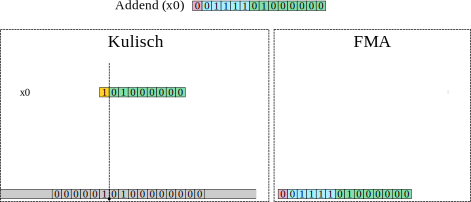
\includegraphics[width=0.8\textwidth]{kulisch1.pdf}
            %\caption{Description for Image 1}
        \end{figure}
    }

    % Show second image on the second slide
    \only<2>{
        \begin{figure}[H]
            \centering
            \includegraphics[width=0.8\textwidth]{kulisch2.pdf}
            %\caption{Description for Image 2}
        \end{figure}
    }

    % Show third image on the third slide
    \only<3>{
        \begin{figure}[H]
            \centering
            \includegraphics[width=0.8\textwidth]{kulisch3.pdf}
            %\caption{Description for Image 3}
        \end{figure}
    }

    % Show fourth image on the fourth slide
    \only<4>{
        \begin{figure}[H]
            \centering
            \includegraphics[width=0.8\textwidth]{kulisch4.pdf}
            %\caption{Description for Image 4}
        \end{figure}
    }
    \only<5->{
        \small
         \begin{exampleblock}<5->{Results}
            \vspace{-6mm}
            \begin{align*}
                R_\text{exact} &= 46.89794921875 \\
                R_\text{FMA} &= 4\color{red}{5.4375} \\
                R_\text{Kulisch} &= 46.89794921875
            \end{align*}
            %\vspace{-12mm}
        \end{exampleblock}

    %    \begin{alertblock}<6->{Error Analysis and Formulas}
    %        \vspace{-6mm}
    %        \begin{align*}
    %            \text{Absolute Error} &= |R_\text{exact} - R| \\
    %            \text{Relative Error} &= \frac{|R_\text{exact} - R|}{|R_\text{exact}|}
    %        \end{align*}

    %        %\vspace{-4mm}
    %        \begin{table}[H]
    %            \centering
    %            \begin{tabular}{|c|c|c|}
    %                \hline
    %                & \textbf{Absolute Error} & \textbf{Relative Error} \\ \hline
    %                \textbf{FMA} & 1.46044921875 & 0.0311 (3.11\%) \\ \hline
    %                \textbf{Kulisch} & 0 & 0 \\ \hline
    %            \end{tabular}
    %        \end{table}
    %    \end{alertblock}
    }
    %\normalsize
\end{frame}



%\begin{frame}
%    \frametitle{Background: Posit format}
%	\begin{columns}
%	\begin{column}{0.5\textwidth}
%		\begin{itemize}
%			\item TEMP
%		\end{itemize}
%	\end{column}
%	\begin{column}{0.5\textwidth}
%    \begin{figure}[H]
%    \centering
%    \begin{figure}{0.65\textwidth}
%        \centering
%        \includegraphics[width=\linewidth]{Chapter2/Figs/posit_16_4_bit_pattern.pdf}
%        \caption{Bit pattern with all components}
%    \end{figure}
%    \\
%    %\hfill
%    \begin{figure}{0.65\textwidth}
%        \centering
%        \includegraphics[width=\linewidth]{Chapter2/Figs/posit_16_4_bit_pattern_no_frac.pdf}
%        \caption{Without fraction}
%    \end{figure}
%    \\
%    \begin{figure}{0.65\textwidth}
%        \centering
%        \includegraphics[width=\linewidth]{Chapter2/Figs/posit_16_4_bit_pattern_no_frac_no_scale.pdf}
%        \caption{Without fraction and scale}
%    \end{figure}
%    \\
%    %\hfill
%    \begin{figure}{0.65\textwidth}
%        \centering
%        \includegraphics[width=\linewidth]{Chapter2/Figs/posit_16_4_bit_pattern_no_frac_no_scale_no_terminating.pdf}
%        \caption{Without fraction, scale, terminating bit}
%    \end{figure}
%	\end{column}
%\end{figure}
%
%\end{frame}

\begin{frame}
    \frametitle{Background: Posit format}
    \begin{columns}
        \begin{column}{0.45\textwidth}
            \begin{itemize}
		\item<1-> \textbf{``Tapered-Precision''} Posit$\left \langle N,es \right \rangle$.
		\item<1-> N the bitwidth, es exponent size.
		\item<2-> \textbf{Variable-Lenght} fields.
		\item<2-> \textbf{Golomb Rice} regime (r).
		\item<2-> \textbf{Regime} is super-exponent
		\item<3-> \textbf{Quire:} Kulisch in standard.
		\item<3-> \textbf{Claim} to replace \textit{IEEE754}
		\item<3-> \textbf{1} NaN
		\item<3-> \textbf{Dynamic Range} enhanced
		\item<3-> \textbf{Precision around one} enhanced
            \end{itemize}
        \end{column}
        \begin{column}{0.55\textwidth}
		\begin{figure}[H]
            \centering
			\vspace{5pt}
            \includegraphics[width=0.9\textwidth]{posit_16_4_bit_pattern.pdf}
			\vspace{-10pt}
            \caption{All components}

            \includegraphics[width=0.9\textwidth]{posit_16_4_bit_pattern_no_frac.pdf}
			\vspace{-10pt}
            \caption{Without fraction}

            \includegraphics[width=0.9\textwidth]{posit_16_4_bit_pattern_no_frac_no_scale.pdf}
			\vspace{-10pt}
            \caption{Without fraction and scale}

            \includegraphics[width=0.9\textwidth]{posit_16_4_bit_pattern_no_frac_no_scale_no_terminating.pdf}
			\vspace{-10pt}
            \caption{Only regime}
	\end{figure}
        \end{column}
    \end{columns}
\end{frame}



\section{Accuracy vs. Energy Efficiency}
\graphicspath{{../../../PhD/paper_factory/thesis_louis/Chapter4/Figs/}{../../../PhD/paper_factory/thesis_louis/Chapter3/Figs/}}
\subsection{Executive Summary}
\begin{frame}
    \frametitle{Current Progress}

    % Adding a thematic title for the slide that fits with the chapter
    \centering
    \huge ``A Generator of Numerically-Tailored Accelerators for Batched GEMMs''
    \normalsize

    \vspace{1em} % Add some vertical space before the table of contents

    % Only shows the current section and its subsections, hides everything else
    \tableofcontents[currentsection,
                     subsectionstyle=show/shaded/hide,
                     sectionstyle=show/hide]

    % Explanation of options:
    % - currentsection: Highlights the current section
    % - subsectionstyle=show/show/hide: The current subsection and its siblings in the current section are shown
    % - sectionstyle=show/hide: Shows only the current section, hides other sections
\end{frame}

\begin{frame}
    \frametitle{Executive Summary}
        \begin{alertblock}<1->{General Matrix Multiplication kernel acceleration}
		A \textbf{large variety of scientific applications} rely on \textbf{GEMM} multiplication kernel. The numerical requirements are \textbf{very heterogeneous}, e.g., AI or weather forecasting.
        \end{alertblock}

        \begin{exampleblock}<2->{State-of-the-Art Accelerators}
		Matrix-Matrix Multiplication (MMM) accelerators \textbf{have no focus on precision/accuracy}, but on performance.
        \end{exampleblock}

        \begin{block}<3->{Our Proposal}
		Generation of scalable Systolic Arrays with \textbf{adaptative precision} Processing Elements.
        \end{block}
\end{frame}


\subsection{Systolic Array Generator}
\begin{frame}
    \frametitle{Current Progress}

    % Only shows the current section and its subsections, hides everything else
    \tableofcontents[currentsection,
                     subsectionstyle=show/shaded/hide,
                     sectionstyle=show/hide]

    % Explanation of options:
    % - currentsection: Highlights the current section
    % - subsectionstyle=show/show/hide: The current subsection and its siblings in the current section are shown
    % - sectionstyle=show/hide: Shows only the current section, hides other sections
\end{frame}

\begin{frame}
    \frametitle{Systolic Array Generator: Overview}

    \begin{columns}
        \begin{column}{0.5\textwidth}
            \begin{itemize}
                \item<1-> BLAS level 3 GEMM routine
                \item<1-> Generator 2D Systolic Arrays
                \item<1-> Target agnostic
                \item<2-> Performance:
                \begin{itemize}
		    \item Scalable
                    \item HSSD Extraction scheme
                \end{itemize}
		\item<3-> \textbf{Arithmetic focus}:
                \begin{itemize}
                    \item S3: Computer format agnostic
		    \item 3 Accumulators
                \end{itemize}
            \end{itemize}
        \end{column}

        \begin{column}{0.5\textwidth}
	    \begin{figure}[H]
            \centering
            \includegraphics[width=\textwidth]{overall_SA_2.pdf}
            \caption{$3 \times 3$ Systolic Array.}
            \label{fig:overall_SA}
	    \end{figure}
        \end{column}
    \end{columns}
	%\only<4->{\onlyfootcite{flopoco2}}
\end{frame}


\begin{frame}
\frametitle{Systolic Array Generator: S3 Format}

            \begin{itemize}
		    \item \textbf{S}ign \textbf{S}cale \textbf{S}ignificand
		    \item All our datapaths are in \textbf{S3} format
		    \item \textbf{Arithmetic Agnostic} once translated/mapped
                    \item Simple arithmetic:
			\begin{itemize}
                    		\item necessary and sufficient bits
                    		\item Eliminate redundancy, dual zeros, special cases
			\end{itemize}
                    \item A quintuple format: \textlangle NaN, Sign, Scale, Implicit, Fraction\textrangle
            \end{itemize}
            \begin{table}
                \centering
                \caption{Common computer number formats and their S3 translations.}
		    \vspace{-0.5cm}
                \label{table:s3_examples}
                \resizebox{0.75\textwidth}{!}{%
                \begin{tabular}{@{}lcccll@{}}
                \toprule
                \textbf{Comp. Arith.} & \textbf{Value} & \(\boldsymbol{S3\ \omega S}\) & \textbf{Bias} & \(\boldsymbol{S3\ \omega F}\) & \textbf{S3 Quintuple} \\
                \midrule
                IEEE-754 16 & 0 & 5 & \(2^{\omega S-1}-1=15\) & 10 & \(\langle0,x,xxxxx,0,0000000000\rangle\) \\
                Posit \( \langle 8,0 \rangle \) & 1 & 4 & \((N-2)\cdot2^{es}=6\) & 5 & \(\langle0,0,0110,1,00000\rangle\) \\
                Posit \( \langle 16,2 \rangle \) & NaN & 7 & \((N-2)\cdot2^{es}=56\) & 11 & \(\langle1,x,xxxxxxx,x,xxxxxxxxxxx\rangle\) \\
                bfloat16 & 3.5 & 8 & \(2^{\omega S-1}-1=127\) & 7 & \(\langle0,0,10000000,1,1100000\rangle\) \\
                \bottomrule
                \end{tabular}
                }
            \end{table}

\end{frame}

%frame:
%A2S3: Arithmetic to S3​
% as long as this unit exist the whole array is uasble, one can come up with a new artihmtic format and this unit to translate into SA
%PEs: Processing Elements​
% the building block cotnraining the FDP unit
%S3FDP: S3 Fused Dot Product​
%
%L2A: Large Accumulator to Arithmetic
% can round (only once at final step)in inptu format or another format, give result as is for exactness
%        \begin{column}{0.5\textwidth}
%	    \begin{figure}[H]
%            \centering
%            \includegraphics[width=\textwidth]{overall_SA_2.pdf}
%            \caption{$3 \times 3$ Systolic Array.}
%            \label{fig:overall_SA}
%	    \end{figure}

%\begin{frame}
%    \frametitle{Systolic Array Components Overview}
%
%    \begin{columns}
%    \begin{column}{0.5\textwidth}
%    \begin{itemize}
%        \item<1-> \textbf{A2S3: Arithmetic to S3}
%        \begin{itemize}
%            \item Translates any arithmetic format into S3, ensuring the array's adaptability.
%        \end{itemize}
%
%        \item<2-> \textbf{PEs: Processing Elements}
%        \begin{itemize}
%            \item Fundamental blocks containing the Fused Dot Product (FDP) unit.
%        \end{itemize}
%
%        \item<3-> \textbf{S3FDP: S3 Fused Dot Product}
%        \begin{itemize}
%            \item Handles dot product calculations within the S3 format.
%        \end{itemize}
%
%        \item<4-> \textbf{L2A: Large Accumulator to Arithmetic}
%        \begin{itemize}
%            \item Rounds only at the final step to maintain precision, outputs in input format or another chosen format for exactness.
%        \end{itemize}
%    \end{itemize}
%    \end{column}
%
%    \begin{column}{0.5\textwidth}
%    \begin{figure}[H]
%        \centering
%        \includegraphics[width=0.5\textwidth]{overall_SA_2.pdf} % Adjust the image width as needed
%        \caption{$3 \times 3$ Systolic Array illustrating key components.}
%        \label{fig:overall_SA}
%    \end{figure}
%        \end{column}
%    \end{columns}
%
%\end{frame}
%
\begin{frame}
    \frametitle{Systolic Array: Building Blocks}

    \begin{columns}
        \begin{column}{0.45\textwidth}
            \begin{itemize}
		    \item<1->\textbf{A2S3}: Arithmetic to S3 - Translates any arithmetic format into \textbf{S3}
		    \item<2->\textbf{PEs}: Processing Elements - Include the \textbf{S3} Fused Dot Product (\textbf{S3FDP})
		    \item<3->\textbf{L2A}: Large Accumulator to Arithmetic - output results in the chosen format (\textbf{exact}, \textbf{same}, \textbf{specific}).
            \end{itemize}
        \end{column}

        \begin{column}{0.55\textwidth}
            \centering
            \only<1>{
            \includegraphics[width=\textwidth]{overall_SA_a2s3.png}
            \caption{Systolic Array key components.\\ $n+m$ "A2S3"}
            }
            \only<2>{
            \includegraphics[width=\textwidth]{overall_SA_PE.png}
            \caption{Systolic Array key components.\\ $n*m$ "PE"}
            }
            \only<3>{
            \includegraphics[width=\textwidth]{overall_SA_l2a.png}
            \caption{Systolic Array key components.\\ $m$ "L2A"}
            }
        \end{column}
    \end{columns}

\end{frame}

\begin{frame}
	\frametitle{Processing Element (PE)}

    \begin{columns}
        \begin{column}{0.6\textwidth}
	\begin{figure}[H]
		\centering
		%\includegraphics[width=\columnwidth]{figs/PE.pdf}
		\includegraphics[width=0.8\textwidth]{PE_S3.pdf}
		\vspace{-0.3cm}
		\caption{Schematic of a PE. HSSD highlighted.}
		%\vspace{-0.6cm}
	\end{figure}

        \end{column}

        \begin{column}{0.4\textwidth}
	    \begin{figure}[H]
            \centering
            \includegraphics[width=\textwidth]{alg_pe.png}
            \caption{}
	    \end{figure}
        \end{column}
    \end{columns}

\end{frame}

\begin{frame}
	\frametitle{S3 Fused-Dot-Product (S3FDP)}

    Adaptative Kulisch Fixed-Point Accumulator~\cite{de_dinechin_fpga-specific_2008}
    \begin{columns}
        \begin{column}{0.55\textwidth}
	    \begin{enumerate}
		\item<1-> Exact Product into extended S3
		\item<2-> S3 translation and alignment to fixed-point
		\item<3-> Accumulation with RCA or CSA (radix-$2^{k}$ approach)
	    \end{enumerate}

        \end{column}

        \begin{column}{0.45\textwidth}
	    \begin{figure}[H]
            \centering
	    \vspace{0.2cm}
            \includegraphics[width=0.69\textwidth]{S3FDP.pdf}
	    \vspace{-0.3cm}
            \caption{Circuit design of a generic S3FDP}
	    \end{figure}
        \end{column}
    \end{columns}

    %\only<1->{\onlyfootcite{de_dinechin_fpga-specific_2008}}

\end{frame}

\subsection{Evaluation}
\begin{frame}
    \frametitle{Current Progress}

    % Only shows the current section and its subsections, hides everything else
    \tableofcontents[currentsection,
                     subsectionstyle=show/shaded/hide,
                     sectionstyle=show/hide]

    % Explanation of options:
    % - currentsection: Highlights the current section
    % - subsectionstyle=show/show/hide: The current subsection and its siblings in the current section are shown
    % - sectionstyle=show/hide: Shows only the current section, hides other sections
\end{frame}


\begin{frame}
    \frametitle{Design Space Exploration (DSE)}

	\begin{alertblock}<1->{\textbf{22} arithmetic formats}
	bfloat16, "ieee8", ieee16, ieee32, ieee64, tfp8, tfp16, tfp32, tfp64, posit<4,0>, posit<8,0>, posit<8,1>, posit<8,2>, posit<16,0>, posit<16,1>, posit<16,2>, posit<32,0>, posit<32,1>, posit<32,2>, posit<64,1>, posit<64,2>, posit<64,3>.
    \end{alertblock}

	\begin{alertblock}<2->{\textbf{3} Accumulator Configurations}
        $\alpha$ - Small accumulator with small MSB for AI; $\beta$ - Exact accumulator (Kulisch and Quire), preventing roundoff errors; $\gamma$ - 100-bit accumulator.
    \end{alertblock}

    \begin{block}<3->{Combinations}
        \textbf{A total of \textbf{66} combinations (arithmetic, accumulator)} explored in our design space exploration.
    \end{block}
\end{frame}

\begin{frame}
    \frametitle{Design Space Exploration Results}

    %\begin{columns}
        %\begin{column}{0.5\textwidth}
%            \begin{itemize}
%                %\item Beta accumulators resources scale quadratically w-r-t the exponent size
%                %\item Table below shows resource and power for IEEE formats for our designs against Xilinx IP FMAs
%            \end{itemize}
        %\end{column}

        %\begin{column}{0.5\textwidth}
            \begin{figure}
                \centering
                \includegraphics[width=0.85\textwidth]{resource_250.png}
                \caption{Routed resource of S3FDPs@250MHz}
                \label{fig:resource_utilization}
            \end{figure}
        %\end{column}
    %\end{columns}

\end{frame}
\begin{frame}{IEEE754 comparison}
    Hardware cost of "IEEE754" S3 vs. Xilinx FMA IP.
    \begin{columns}

        % Column 1
        \begin{column}{0.5\textwidth}
%            % 8-bit Table
%            \begin{table}
%            \caption{8-bit configurations}
%	    \vspace{-0.2cm}
%            \centering
%                \resizebox{0.85\textwidth}{!}{%
%            \begin{tabular}{@{} lcccc @{}}
%                \toprule
%		    Config. & \cellcolor{green!25}$\alpha$ & $\beta$ & $\gamma$ & \textit{FMA} \\
%                \midrule
%		    LUTs & 85 & 109 & 166 & 233 \\
%                FFs  & 18 & 42  & 102 & 342 \\
%                DSPs & 0  & 0   & 0   & 1   \\
%                CARRY8s & 2  & 6   & 13  & 17  \\
%                Power(PE)(W) & 0.003 & 0.004 & 0.006 & 0.016 \\
%                Power(system)(W) & 2.828 & 4.807 & 9.860 & 15.872 \\
%                En. Eff.(system)(GFlops/s/W) & 175.4 & 103.2 & 50.3 & 31.3 \\
%                \bottomrule
%            \end{tabular}
%		    }
%            \end{table}
		\begin{table}
		\caption{8-bit configurations}
		\vspace{-0.2cm}
		\centering
		\resizebox{0.85\textwidth}{!}{%
		\begin{tabular}{@{} lcccc @{}}
		    \toprule
		    Config. & $\alpha$ & $\beta$ & $\gamma$ & \textit{FMA} \\
		    \midrule
		    LUTs & \cellcolor{green!25}85 & \cellcolor{yellow!25}109 & \cellcolor{orange!25}166 & \cellcolor{red!25}233 \\
		    FFs  & \cellcolor{green!25}18 & \cellcolor{yellow!25}42  & \cellcolor{orange!25}102 & \cellcolor{red!25}342 \\
		    DSPs & \cellcolor{green!25}0  & \cellcolor{green!25}0   & \cellcolor{green!25}0   & \cellcolor{red!25}1   \\
		    CARRY8s & \cellcolor{green!25}2 & \cellcolor{yellow!25}6 & \cellcolor{orange!25}13 & \cellcolor{red!25}17  \\
		    Power(PE)(W) & \cellcolor{green!25}0.003 & \cellcolor{yellow!25}0.004 & \cellcolor{orange!25}0.006 & \cellcolor{red!25}0.016 \\
		    Power(system)(W) & \cellcolor{green!25}2.828 & \cellcolor{yellow!25}4.807 & \cellcolor{orange!25}9.860 & \cellcolor{red!25}15.872 \\
		    En. Eff.(system)(GFlops/s/W) & \cellcolor{green!25}175.4 & \cellcolor{yellow!25}103.2 & \cellcolor{orange!25}50.3 & \cellcolor{red!25}31.3 \\
		    \bottomrule
		\end{tabular}
		}
		\end{table}
	    \begin{table}
		\caption{32-bit configurations}
		\vspace{-0.2cm}
		\centering
		\resizebox{0.85\textwidth}{!}{%
		\begin{tabular}{@{} lcccc @{}}
		    \toprule
		    Config. & $\alpha$ & $\beta$ & $\gamma$ & \textit{FMA} \\
		    \midrule
		    LUTs & \cellcolor{green!25}345 & \cellcolor{red!25}1039 & \cellcolor{yellow!25}416 & \cellcolor{orange!25}769 \\
		    FFs  & \cellcolor{green!25}225 & \cellcolor{orange!25}865  & \cellcolor{yellow!25}317 & \cellcolor{red!25}1278 \\
		    DSPs & \cellcolor{green!25}2   & \cellcolor{green!25}2    & \cellcolor{green!25}2   & \cellcolor{green!25}2    \\
		    CARRY8s & \cellcolor{green!25}12 & \cellcolor{yellow!25}19  & \cellcolor{orange!25}37  & \cellcolor{red!25}73  \\
		    Power(PE)(W) & \cellcolor{green!25}0.019 & \cellcolor{orange!25}0.058 & \cellcolor{yellow!25}0.023 & \cellcolor{red!25}0.066 \\
		    Power(system)(W) & \cellcolor{green!25}1.233 & \cellcolor{red!25}5.329 & \cellcolor{yellow!25}1.554 & \cellcolor{orange!25}3.696 \\
		    En. Eff.(system)(GFlops/s/W) & \cellcolor{green!25}22.7 & \cellcolor{red!25}5.6 & \cellcolor{yellow!25}18.09 & \cellcolor{orange!25}7.6 \\
		    \bottomrule
		\end{tabular}
		}
		\end{table}


        \end{column}

        % Column 2
        \begin{column}{0.5\textwidth}
            % 16-bit Table
%            \begin{table}
%            \caption{16-bit configurations}
%	    \vspace{-0.2cm}
%            \centering
%                \resizebox{0.85\textwidth}{!}{%
%            \begin{tabular}{@{} lcccc @{}}
%                \toprule
%                Config. & \cellcolor{green!25}$\alpha$ & $\beta$ & $\gamma$ & \textit{FMA} \\
%                \midrule
%                LUTs & 134 & 187 & 200 & 425 \\
%                FFs  & 34  & 124 & 102 & 680 \\
%                DSPs & 1   & 1   & 1   & 1   \\
%                CARRY8s & 4  & 16  & 13  & 22  \\
%                Power(PE)(W) & 0.008 & 0.018 & 0.014 & 0.032 \\
%                Power(system)(W) & 2.121 & 3.177 & 3.749 & 7.680 \\
%                En. Eff.(system)(GFlops/s/W) & 56.6 & 37.8 & 32.0 & 15.6 \\
%                \bottomrule
%            \end{tabular}
%		    }
%            \end{table}

		\begin{table}
		\caption{16-bit configurations}
		\vspace{-0.2cm}
		\centering
		\resizebox{0.85\textwidth}{!}{%
		\begin{tabular}{@{} lcccc @{}}
		    \toprule
		    Config. & $\alpha$ & $\beta$ & $\gamma$ & \textit{FMA} \\
		    \midrule
		    LUTs & \cellcolor{green!25}134 & \cellcolor{yellow!25}187 & \cellcolor{orange!25}200 & \cellcolor{red!25}425 \\
		    FFs  & \cellcolor{green!25}34  & \cellcolor{yellow!25}124 & \cellcolor{orange!25}102 & \cellcolor{red!25}680 \\
		    DSPs & \cellcolor{green!25}1   & \cellcolor{green!25}1   & \cellcolor{green!25}1   & \cellcolor{green!25}1   \\
		    CARRY8s & \cellcolor{green!25}4  & \cellcolor{yellow!25}16 & \cellcolor{orange!25}13 & \cellcolor{red!25}22  \\
		    Power(PE)(W) & \cellcolor{green!25}0.008 & \cellcolor{orange!25}0.018 & \cellcolor{yellow!25}0.014 & \cellcolor{red!25}0.032 \\
		    Power(system)(W) & \cellcolor{green!25}2.121 & \cellcolor{yellow!25}3.177 & \cellcolor{orange!25}3.749 & \cellcolor{red!25}7.680 \\
		    En. Eff.(system)(GFlops/s/W) & \cellcolor{green!25}56.6 & \cellcolor{yellow!25}37.8 & \cellcolor{orange!25}32.0 & \cellcolor{red!25}15.6 \\
		    \bottomrule
		\end{tabular}
		}
		\end{table}

            % 64-bit Table
%            \begin{table}
%            \caption{64-bit configurations}
%	    \vspace{-0.2cm}
%            \centering
%                \resizebox{0.85\textwidth}{!}{%
%            \begin{tabular}{@{} lcccc @{}}
%                \toprule
%                Config. & \cellcolor{green!25}$\alpha$ & $\beta$ & $\gamma$ & \textit{FMA} \\
%                \midrule
%                LUTs        & 1806 & 11414 & 1668 & 1785 \\
%                FFs         & 1383 & 8996  & 1089 & 2884 \\
%                DSPs        & 6    & 6     & 6    & 10   \\
%                CARRY8s     & 38   & 272   & 34   & 70   \\
%                Power(PE)(W) & 0.085 & 0.460 & 0.081 & 0.191 \\
%                Power(system)(W) & 1.002 & 13.633 & 0.971 & 2.292 \\
%                En. Eff.(system)(GFlops/s/W) & 6.0 & 0.4 & 6.2 & 2.6 \\
%                \bottomrule
%            \end{tabular}
%		    }
%            \end{table}

	    \begin{table}
		\caption{64-bit configurations}
		\vspace{-0.2cm}
		\centering
		\resizebox{0.85\textwidth}{!}{%
		\begin{tabular}{@{} lcccc @{}}
		    \toprule
		    Config. & $\alpha$ & $\beta$ & $\gamma$ & \textit{FMA} \\
		    \midrule
		    LUTs        & \cellcolor{orange!25}1806 & \cellcolor{red!25}11414 & \cellcolor{green!25}1668 & \cellcolor{yellow!25}1785 \\
		    FFs         & \cellcolor{yellow!25}1383 & \cellcolor{red!25}8996  & \cellcolor{green!25}1089 & \cellcolor{orange!25}2884 \\
		    DSPs        & \cellcolor{green!25}6    & \cellcolor{green!25}6    & \cellcolor{green!25}6    & \cellcolor{red!25}10   \\
		    CARRY8s     & \cellcolor{yellow!25}38   & \cellcolor{red!25}272   & \cellcolor{green!25}34   & \cellcolor{orange!25}70   \\
		    Power(PE)(W) & \cellcolor{yellow!25}0.085 & \cellcolor{red!25}0.460 & \cellcolor{green!25}0.081 & \cellcolor{orange!25}0.191 \\
		    Power(system)(W) & \cellcolor{yellow!25}1.002 & \cellcolor{red!25}13.633 & \cellcolor{green!25}0.971 & \cellcolor{orange!25}2.292 \\
		    En. Eff.(system)(GFlops/s/W) & \cellcolor{yellow!25}6.0 & \cellcolor{red!25}0.4 & \cellcolor{green!25}6.2 & \cellcolor{orange!25}2.6 \\
		    \bottomrule
		\end{tabular}
		}
		\end{table}
	\end{column}

    \end{columns}
\end{frame}

\begin{frame}
    \frametitle{DSE: Scalability of PnR designs}

    \begin{columns}
        \begin{column}{0.5\textwidth}
            \begin{figure}
                \centering
                \includegraphics[width=0.95\columnwidth]{art_gallery_sa_32_31_8_0_by_PE_highlight.png}
                \caption{\(32 \times 31\) \(posit \langle 8,1 \rangle \beta\) array}
            \end{figure}
        \end{column}

        \begin{column}{0.5\textwidth}
            \begin{figure}
                \centering
                \includegraphics[width=0.95\columnwidth]{art_gallery_sa_64_63_4_0_by_col_highlight.png}
                \caption{\(64 \times 63\) \(posit \langle 4,0 \rangle \beta\) array}
            \end{figure}
        \end{column}
    \end{columns}

\end{frame}

\begin{frame}
    \frametitle{Hardware Platform Overview}

    \begin{columns}
        \begin{column}{0.5\textwidth}
            \begin{itemize}
                \item Power9 System (IBM AC922 with AlphaData 9V3 FPGA Board):
                \begin{itemize}
                    \item XCVU3P-2-FFVC1517 FPGA, UltraScale+ family.
                    \item AC922 POWER9 system, 40 cores (20 per socket), 2.3GHz.
                \end{itemize}
                \item FPGA Specifications:
                \begin{itemize}
                    \item LUTs: 384k
                    \item Flip-Flops: 788k
                    \item DSP Slices: 2280
                    \item Block RAM: 25.3Mb
                    \item UltraRAM: 90Mb
                \end{itemize}
                \item PCIe Gen4-8 lanes, 15.754 GB/s, supports CAPI2 and IBM SNAP.
            \end{itemize}
        \end{column}

        \begin{column}{0.5\textwidth}
	    \begin{figure}[H]
            \centering
            \includegraphics[width=\textwidth]{p9.png}
            \caption{IBM Power9 AC922 ; CAPI2 + VU3P.}
	    \end{figure}
        \end{column}
    \end{columns}

\end{frame}

%Title: Evaluation
%
%To evaluate generated accelerators, we consider:​
%
%Throughput (B/s)​
%
%Performance (Ops/s)​
%
%Energy Efficiency (Ops/s/W)​
%
%Accuracy (number of accurate bits)​
%
%Below, we observe throughput and performance for different arrays
%\begin{figure}[H]
%  \centering
%  \includegraphics[width=\columnwidth]{throughput.pdf}
%  %\vspace{-0.9cm}
%  \vspace{-0.6cm}
%	\caption{Measured and averaged vs theoretical Throughput (GBytes/s) for different Payload Sizes (Bytes).}
%  \label{fig:throughput}
%  %\vspace{-0.5cm}
%\end{figure}
%\begin{figure}[H]
%  \centering
%  \includegraphics[width=0.8\columnwidth]{performance.pdf}
%  %\vspace{-0.9cm}
%  %\vspace{-0.6cm}
%	\caption{Measured and theoretical Performances for different array sizes and Payload Sizes.}
%  %\vspace{1.0cm}
%  \label{fig:performance}
%  %\vspace{-0.7cm}
%\end{figure}


\begin{frame}
    \frametitle{Evaluation: Energy Efficiency VS Accuracy}

    %\begin{columns}
        %\begin{column}{0.35\textwidth}
        %\end{column}

        %\begin{column}{0.65\textwidth}
            \begin{figure}
                \centering
                \includegraphics[width=0.85\textwidth]{accuracy_energy_eff_bitwidth.pdf}
		\vspace{-2mm}
                \caption{Energy efficiency (top) against Accuracy (bottom)}
                \label{fig:accuracy}
            \end{figure}
        %\end{column}
    %\end{columns}

%\only<1->{\onlyfootcite{fousse_mpfr_2007}}
\note[item]{Uniform distribution between -1 and 1.}
\note[item]{10 averaged runs.}
\note[item]{Accuracy log2 of relative error against mpfr}
\note[item]{FMA in lighter lines}
\note[item]{$\beta$ is costly but precise}
\note[item]{FMA is less accurate and costs more than FDP}

\end{frame}

\begin{frame}
    \frametitle{Zoom on 16-bit: Energy Efficiency VS Accuracy}
     \begin{figure}
         \centering
         \includegraphics[width=\textwidth]{zoom_16bits.png}
         %\vspace{-2mm}
         \caption{Energy eff. and Accuracy for different payload sizes.}
         \label{fig:accuracy}
     \end{figure}

\end{frame}

\subsection{Conclusions}
\begin{frame}
    \frametitle{Current Progress}

    % Only shows the current section and its subsections, hides everything else
    \tableofcontents[currentsection,
                     subsectionstyle=show/shaded/hide,
                     sectionstyle=show/hide]

    % Explanation of options:
    % - currentsection: Highlights the current section
    % - subsectionstyle=show/show/hide: The current subsection and its siblings in the current section are shown
    % - sectionstyle=show/hide: Shows only the current section, hides other sections
\end{frame}

\begin{frame}
    \frametitle{Summary of Insights and Key Contributions}
        \begin{alertblock}<1->{Large Design Space Exploration}
		Conducting extensive design space exploration and evaluation leading to \textbf{several profiles of GEMM kernels}.
        \end{alertblock}
	\vspace{-3mm}

        \begin{block}<2->{State-of-the-art Enhancement}
		Improving single-precision energy efficiency of FPGA GEMM accelerators by \textbf{1.86$\times$}.
        \end{block}
	\vspace{-3mm}

        \begin{block}<3->{Answering Sparsity of numerical Requirements}
		Our accelerators achieve \textbf{240 GOps/s/W with 4 accurate} bits to \textbf{0.65 GOps/s/W with over 1000} accurate bits, serving a \textbf{broad range of applications}.
        \end{block}
	\vspace{-3mm}

        \begin{exampleblock}<4->{Findings}
		Internal \textbf{precision budgeting} against a workload \textbf{alleviates "the walls"}.
        \end{exampleblock}

\end{frame}
\begin{frame}
    \frametitle{Discussions}


   \begin{block}<1->{Workload Discussion}
	   The range \([-1, 1]\) does not reflect real workload conditions. Other contributions propose evaluations with \textbf{artificial} matrices in ranges like \([-10, 10]\), \([-100, 100]\), up to \([-10^{8}, 10^{8}]\).
    \end{block}

        \begin{block}<2->{Future Research Directions}
            Adopt a more \textbf{realistic} approach by bridging to software-based HPC code.
        \end{block}
\end{frame}

\graphicspath{{../../../PhD/paper_factory/thesis_louis/Chapter5/Figs/}}
%\subsection{Executive Summary}
%\begin{frame}
%    \frametitle{Current Progress}
%
%    % Adding a thematic title for the slide that fits with the chapter
%    \centering
%    \huge ``An Open-Source Framework for Efficient Numerically-Tailored Computations''
%    \normalsize
%
%    \vspace{1em} % Add some vertical space before the table of contents
%
%    % Only shows the current section and its subsections, hides everything else
%    \tableofcontents[currentsection,
%                     subsectionstyle=show/shaded/hide,
%                     sectionstyle=show/hide]
%
%    % Explanation of options:
%    % - currentsection: Highlights the current section
%    % - subsectionstyle=show/show/hide: The current subsection and its siblings in the current section are shown
%    % - sectionstyle=show/hide: Shows only the current section, hides other sections
%\end{frame}
%
%
%\begin{frame}
%    \frametitle{Executive Summary}
%
%    % Uncover each block one by one
%        \begin{block}<1->{GEMM Multiplication Kernel}
%		A large variety of scientific applications rely on \textbf{GEMM } kernel. The \textbf{numerical requirements are very heterogeneous}, e.g., AI or weather forecasting.
%        \end{block}
%
%        \begin{exampleblock}<2->{Lack of Hardware Precision Adaptability}
%		\textbf{Extended} or adaptative \textbf{software precision is expensive} and often the computations land in commodity hardware.
%        \end{exampleblock}
%
%        \begin{alertblock}<3->{Our Proposal}
%		We propose an \textbf{Open-Source framework} to bridge high-level libraries to numerically aware and accelerated GEMM kernels.
%        \end{alertblock}
%\end{frame}

\subsection{Bridging to real workloads}
\subsubsection{Open Source SW/HW Co-designed Framework}
\begin{frame}
    \frametitle{Current Progress}

    % Only shows the current section and its subsections, hides everything else
    \tableofcontents[currentsection,
                     subsectionstyle=show/shaded/hide,
                     sectionstyle=show/hide]

    % Explanation of options:
    % - currentsection: Highlights the current section
    % - subsectionstyle=show/show/hide: The current subsection and its siblings in the current section are shown
    % - sectionstyle=show/hide: Shows only the current section, hides other sections
\end{frame}

\begin{frame}
    \frametitle{Open Source SW/HW Co-designed Framework}
    \begin{figure}
      \centering
      \includegraphics[width=\textwidth]{overall_framework.pdf}
      \caption{The 2 phases of the framework: right, the a priori Hardware generation flow, and left, the runtime execution flow.}
    \end{figure}

\end{frame}


\begin{frame}
    \frametitle{Framework: Hardware Side}

    \begin{columns}

    \begin{column}{0.5\textwidth} % Adjust width as needed
        \begin{itemize} % Incremental overlay specifications
	    \item<1-> Configuration files to bitstream
	    \item<1-> Modified FloPoCo~\cite{flopoco1}
            \item<1-> OpenCAPI offers $\approx$23GBp/s with 1024-bit bus @200MHz
        \end{itemize}
    \end{column}

    \begin{column}{0.5\textwidth}
        \begin{figure}
            \centering
            \includegraphics[width=\textwidth]{framework_HW.pdf}
            \caption{Automated HW generation}
        \end{figure}
    \end{column}

    \end{columns}

\onlyfootcite{flopoco1}

\end{frame}

\begin{frame}
    \frametitle{Framework: Software Side}

    \begin{columns}

    \begin{column}{0.35\textwidth} % Adjust width as needed
	\only<1>{
	Strategy:
        \begin{itemize}
		\item<1-> HPC codes rely on \textbf{BLAS calls}
		\item<1-> \textbf{Numpy, Pytorch}
		\item<1-> Intercept, cast, dispatch
        \end{itemize}
	}
	\only<2>{
	\begin{itemize}

        	% User Process items
        	\item \textbf{User Process:}
        	\begin{enumerate}
        	    \item Matrix Allocation
        	    \item Call \texttt{gemm()}
        	\end{enumerate}

        	% Spacer
        	\vspace{1em}

        	% Our Library items
        	\item \textbf{Our lib:}
        	\begin{enumerate}
		    \setcounter{enumi}{2}
        	    \item Arithmetic cast
        	    \item Signal DMA properties
        	    \item HW address translation
        	    \item DMA starts
        	\end{enumerate}
    \end{itemize}
    }
    \end{column}

    \begin{column}{0.65\textwidth}
        \begin{figure}
            \centering
            \includegraphics[width=\textwidth]{framework_SW.pdf}
            \caption{Software flow}
        \end{figure}
    \end{column}

    \end{columns}

\end{frame}

\begin{frame}
	\frametitle{SW Code Example}

	\small
    \begin{figure}
        \centering
        \includegraphics[width=0.8\textwidth]{listing1.png}
	    \vspace{-3mm}
        \caption{Calling twice the same user application (python) with our BLAS}
    \end{figure}
	    \vspace{-2mm}

    \begin{figure}
        \centering
        \includegraphics[width=0.8\textwidth]{listing2.png}
	    \vspace{-3mm}
        \caption{gemm.py: a python program calling GEMMs. No changes in the code.}
    \end{figure}
	\normalsize

\end{frame}

\subsubsection{Workload Evaluation}
\begin{frame}
    \frametitle{Current Progress}

    % Only shows the current section and its subsections, hides everything else
    \tableofcontents[currentsection,
                     subsectionstyle=show/shaded/hide,
                     sectionstyle=show/hide]

    % Explanation of options:
    % - currentsection: Highlights the current section
    % - subsectionstyle=show/show/hide: The current subsection and its siblings in the current section are shown
    % - sectionstyle=show/hide: Shows only the current section, hides other sections
\end{frame}

\begin{frame}
	\frametitle{Evaluation of HPC Codes: Sea Surface Height (SSH)}

%\scriptsize

\begin{columns}

\begin{column}{0.5\textwidth}
    \begin{myitemize}
        \item<1-> Ocean circulation models
	\item<1-> Monitors climate changes~\cite{barrick_ocean}
	\item<1-> \textbf{Precision-hungry} workload
	\item<1-> Alternating signs and spans over \textbf{15 orders of magnitude}
	\item<1-> Can be solved without hardware
	\item<1-> Kahan SCS, DCS~\cite{kahan_pracniques_1965}
	\item<1-> Extended Software Precision~\cite{bailey_high-precision_2009})
    \end{myitemize}
\end{column}
\begin{column}{0.5\textwidth}
    \begin{figure}
	    \vspace{2mm}
        \includegraphics[width=\textwidth]{4_forloops.pdf}
	    \vspace{-11mm}
	    \caption{Double-precision errors.}
    \end{figure}
\end{column}

\end{columns}


\onlyfootcite{barrick_ocean}
\onlyfootcite{kahan_pracniques_1965}
\onlyfootcite{bailey_high-precision_2009}
\normalsize

	\note[item]  {(conv, im2col, FC)}

\end{frame}

\begin{frame}
\frametitle{Evaluation of HPC Codes: Artificial Intelligence}

%\scriptsize

\begin{columns}

\begin{column}{0.5\textwidth}
    %\textbf{Artificial Intelligence (AI)}
    \begin{myitemize}
	\item GEMMs (im2col, FC, Conv)
        %\item Used to solve many modern problems (image recognition, NLP)
	\item \textbf{Precision-resilient} workloads~\cite{johnson_rethinking_2018}
        \item Accumulations of closely related values~\cite{li_robustness-aware_2021}
    \end{myitemize}
    %\vspace{-2mm} % Adjust spacing as needed
\end{column}
\begin{column}{0.5\textwidth}
    \begin{figure}
        \includegraphics[width=\textwidth]{histograms.jpg}
	    \caption{Weights histograms Alexnet/Resnet18}
    \end{figure}
\end{column}
\end{columns}


\onlyfootcite{li_robustness-aware_2021}
\onlyfootcite{johnson_rethinking_2018}
\normalsize

	\note[item]  {(conv, im2col, FC)}

\end{frame}

\begin{frame}
\frametitle{Evaluation: SSH results}

\begin{columns}

\begin{column}{0.5\textwidth}
	\tiny
%\scriptsize
\begin{myitemize}
	\item<1-> \textbf{IEEE754-64-FDP} vs. \textbf{IEEE754-64/128 FMAs}
	\tiny
    \begin{myitemize}
	\tiny
        \item 64-bit format + 91-bit FDP: <ovf:30,msb:30,lsb:-30>
	\item 128-bit quad-precision FMA
        \item 64-bit double-precision FMA
    \end{myitemize}
	\item<2-> \textbf{10 shuffles} per chunk size
	\item<2-> \textbf{4 metrics}: mean, RSD, Accuracy, Accuracy cost
    \tiny
    \item<3-> The FDP maintains \textbf{reproducibility} unlike the FMA
    \item<3-> The FDP always exhibits \textbf{52} correct bits
    \begin{myitemize}
	\tiny
	\item \textbf{5x} better than quad-precision
	\item \textbf{27.7x} better than double-precision
    \end{myitemize}

	\tiny
    \item<4-> At 200MHz, power consumptions are:
    \begin{myitemize}
	\tiny
        \item 0.266W for IEEE754-64
        \item 0.549W for IEEE754-128
        \item 0.491W for 91-bit FDP
    \end{myitemize}
	\tiny
    \item<5-> For the same Wattage, our FDP generates:
    \begin{myitemize}
	\tiny
	\item \textbf{5.6x} more correct bits than IEEE754-128
	\item \textbf{15.1x} more correct bits than IEEE754-64
    \end{myitemize}
\end{myitemize}
\end{column}

\tiny
\begin{column}{0.5\textwidth}
\centering
\includegraphics[width=0.85\columnwidth]{SSH.pdf}
\caption{IEEE754-64/128 FMAs vs. [64+91]-FDP}
\end{column}

\end{columns}
\normalsize
\end{frame}

\begin{frame}
\frametitle{Evaluation: AI results}

\begin{columns}

\begin{column}{0.4\textwidth}
\tiny
\begin{itemize}
	\item<1-> \textbf{Pytorch code without any changes}
	\item<1-> Top1/5 scores and \textbf{``score costs''}
	\vspace{3mm}
    \item<2-> Evaluated models:
        \begin{itemize}
\tiny
            \item ResNet18
            \item ResNet34
            \item ResNet50
            \item DenseNet121
            \item DenseNet169
            \item VGG11\_BN
        \end{itemize}
    \item<3-> Evaluated datasets:
        \begin{itemize}
\tiny
            \item CIFAR10
            \item ImageNet
        \end{itemize}
    \item<4-> Evaluated computer formats:
        \begin{itemize}
\tiny
            \item IEEE754-32
            \item BrainFloat16
        \end{itemize}
    \item<5-> 27 accumulators and conventional FMA
    \item<5-> A total of \textbf{384} combinations
\end{itemize}
\end{column}

\begin{column}{0.6\textwidth}
\tiny
\centering
\includegraphics[width=\columnwidth]{nn_accuracy_and_acc_per_power_all_subplot.png}
\caption{Top1/5 scores/costs across different models/formats/datasets/accumulators}
\end{column}

\end{columns}
\normalsize
\end{frame}

\begin{frame}
\frametitle{A zoom on the LSB case}
\begin{figure}
	\centering
	\includegraphics[width=0.75\textwidth]{zoom_accuracy.png}
	\vspace{-10pt}
	\caption{The impact of lowering number of LSBs on Top1/5 scores and score costs.}
\end{figure}
\end{frame}

\begin{frame}
\frametitle{A zoom on the LSB + densenet121 + ImageNet case}
\begin{figure}
	\centering
	\includegraphics[width=0.75\textwidth]{zoom_accuracy_highlight.png}
	\vspace{-10pt}
	\caption{The impact of lowering number of LSBs on Top1/5 scores and score costs.}
\end{figure}
\end{frame}

\begin{frame}
\frametitle{Evaluation: AI results}

\begin{figure}
	\centering
	\includegraphics[width=0.97\columnwidth]{nn_power_all_subplots.pdf}
	\vspace{-4mm}
	\caption{Top1 scores VS. Energy cost of inferencing validation set}
\end{figure}

\normalsize
\end{frame}

\begin{frame}
    \frametitle{Zoom on ImageNet + Resnet50}

	\only<1-4>{
	\begin{figure}[H]
            \centering
		%\vspace{1mm}
	    	\only<1>{
	            	\includegraphics[width=\textwidth]{zoom_imagenet_resnet50.png}
			%\vspace{-2mm}
			\caption{Test Set Inference Cost VS. Top1 Score.}
		}
	    	\only<2>{
	            	\includegraphics[width=\textwidth]{zoom_imagenet_resnet50_2.png}
			%\vspace{-2mm}
			\caption{Test Set Inference Cost VS. Top1 Score.}
		}
	    	\only<3>{
	            	\includegraphics[width=\textwidth]{zoom_imagenet_resnet50_3.png}
			%\vspace{-2mm}
			\caption{Test Set Inference Cost VS. Top1 Score.}
		}
	    	\only<4>{
	            	\includegraphics[width=\textwidth]{zoom_imagenet_resnet50_4.png}
			%\vspace{-2mm}
			\caption{Test Set Inference Cost VS. Top1 Score.}
		}
	\end{figure}
	}
%            \item goal: 84\% top 1 score
%            \item FDP<9,6-20> saves 25Wh for bf16 and 100Wh for FP32


	\only<5>{
        \begin{block}{Graphical Superiority}
		Graphically, it always exists one \textbf{FDP} to the left (indicating lower energy) and are never below (ensuring equal or greater accuracy) conventional FMAs, \textbf{highlighting their superior performance}
        \end{block}
	}
    \normalsize

\end{frame}

\subsection{Conclusions}
\begin{frame}
    \frametitle{Current Progress}

    % Only shows the current section and its subsections, hides everything else
    \tableofcontents[currentsection,
                     subsectionstyle=show/shaded/hide,
                     sectionstyle=show/hide]

    % Explanation of options:
    % - currentsection: Highlights the current section
    % - subsectionstyle=show/show/hide: The current subsection and its siblings in the current section are shown
    % - sectionstyle=show/hide: Shows only the current section, hides other sections
\end{frame}

\begin{frame}
    \frametitle{Summary of Insights and Key Contributions}

	\begin{alertblock}<1->{Open-Source Framework}
		A \textbf{bridge} from user applications to silicon, focusing on \textbf{tailored arithmetic} solutions.
	\end{alertblock}
	\vspace{-2mm}
	\begin{alertblock}<2->{Transparent Integration}
		Seamlessly integrates \textbf{without code modification}, agnostic of underlying hardware.
	\end{alertblock}
	\vspace{-2mm}
	\begin{block}<3->{Enhancing State-of-the-Art}
		Improves \textbf{energy efficiency and accuracy} across \textbf{drastically diverse HPC applications}.
	\end{block}
	\vspace{-2mm}
	\begin{exampleblock}<4->{Findings}
		System-wise Arithmetic and numerically-tailored solutions alleviate the power wall (A), and the concern of workload sparsity (B).
	\end{exampleblock}
\end{frame}

\section{Latency vs. Parallelism}
\graphicspath{{../../../PhD/paper_factory/thesis_louis/Chapter6/Figs/}}
\subsection{Executive Summary}
\begin{frame}
    \frametitle{Current Progress}

    % Adding a thematic title for the slide that fits with the chapter
    \centering
    \huge ``Divisions in Vector Processing: Leveraging Opportunities from a Paradigm Shift''
    \normalsize

    \vspace{1em} % Add some vertical space before the table of contents

    % Only shows the current section and its subsections, hides everything else
    \tableofcontents[currentsection,
                     subsectionstyle=show/shaded/hide,
                     sectionstyle=show/hide]

    % Explanation of options:
    % - currentsection: Highlights the current section
    % - subsectionstyle=show/show/hide: The current subsection and its siblings in the current section are shown
    % - sectionstyle=show/hide: Shows only the current section, hides other sections
\end{frame}

%\begin{frame}
%    \frametitle{Executive Summary: Vector Processing Revival}
%
%\scriptsize
%
%    \only<1->{
%        \begin{block}{Context and Challenges}
%            Vector processing is resurging to address the limitations of dark silicon and the end of Dennard scaling, which challenge scalar architectures. Historically crucial for high-performance computing, vector processing is being revitalized through modern instruction sets like RISC-V's "V" extension and open-source silicon projects.
%        \end{block}
%    }
%
%    \only<2->{
%        \begin{exampleblock}{Contributions and Innovations}
%            This chapter introduces novel division algorithms tailored for vector processing, enhancing latency and throughput trade-offs. We present a custom ASIC flow, facilitating design evaluations across multiple PDKs, which emphasizes our commitment to open-source and efficient hardware design.
%        \end{exampleblock}
%    }
%
%    \only<3->{
%        \begin{alertblock}{Impact and Findings}
%            Our approaches lead to significant area and power efficiencies, allowing for dense and efficient computational architectures. For every evaluated computer format, our methods support the integration of multiple units without performance loss, showcasing substantial improvements in power and area metrics.
%        \end{alertblock}
%    }
%\end{frame}

\begin{frame}
    \frametitle{Executive Summary: Vector Processing Revival}
    \scriptsize



\begin{alertblock}<1->{Opportunity 1: Vector Processing}
	Resurgence of \textbf{vector processing} exemplified by the \textbf{RISC-V "V"} extension. \textbf{Enhance Data-level parallelism (DLP)} by trading \textbf{space and time} implementations.
\end{alertblock}

    \begin{alertblock}<2->{Opportunity 2: Open Source Silicon}
	    The momentum in \textbf{open-source silicon community} facilitates \textbf{tape-outs in academia}.
    \end{alertblock}

    \begin{block}<3->{Algorithmic Contribution: Division Algorithm}
	    Less famous operation but useful: \textbf{N-body simulation}; proposal: \textbf{muliple slower, area/power-efficient} units.
    \end{block}
    \begin{block}<4->{Open ASIC Flow Contribution}
	    \textbf{Custom Open ASIC flow} for \textbf{extensive design space exploration} to characterize the divisions.
    \end{block}


    \note[item]{Vector processing exploits data-level parallelism, which is highly beneficial for processing large datasets common in today's applications. This approach is particularly effective for tasks that require the same operation to be performed simultaneously on multiple pieces of data.}
    \note[item]{With the end of Dennard scaling, improving power efficiency is crucial. Vector processors consume less power per computation compared to scalar processors by reducing the operational overhead associated with executing multiple scalar operations.}
\end{frame}

\subsection{Algorithmic Contribution}
\begin{frame}
    \frametitle{Current Progress}

    % Only shows the current section and its subsections, hides everything else
    \tableofcontents[currentsection,
                     subsectionstyle=show/shaded/hide,
                     sectionstyle=show/hide]

    % Explanation of options:
    % - currentsection: Highlights the current section
    % - subsectionstyle=show/show/hide: The current subsection and its siblings in the current section are shown
    % - sectionstyle=show/hide: Shows only the current section, hides other sections
\end{frame}

\begin{frame}
\frametitle{Algorithmic Proposal}

\begin{columns}
    \begin{column}{0.5\textwidth}
	\only<1->{
	\textbf{Baseline,} n the mantissa size:
        \begin{itemize}
	    \item Non-branching with a single n-bit adder.
            \item n iteration.
        \end{itemize}
	}
	\only<2->{
		\textbf{Unrolling Proposal}:
        \begin{itemize}
	    \item Serial addition of $k$ bits
	    \item $k \in [1;n]$
	    \item Reduces a \textbf{power hungry} section
	    \item Reduces the \textbf{area}
	    \item Introduces slowdown
        \end{itemize}
	}
    \end{column}

    \begin{column}{0.5\textwidth}
        \centering
        \includegraphics[width=0.75\columnwidth]{non_restoring_schematic.pdf}
        \caption{Non-restoring division circuit}
        \label{fig:non_restoring_schematic}
    \end{column}
\end{columns}
\end{frame}

\begin{frame}
    \frametitle{Algorithm Finite State Machine}

    \small
    \begin{columns}
        \begin{column}{0.5\textwidth}
		\begin{figure}
            \centering
            \resizebox{!}{0.75\textheight}{%
                \begin{tikzpicture}[>=stealth,shorten >=1pt,auto,node distance=2.8cm]
                    \node[initial,state] (IDLE)      {IDLE};
                    \node[state]         (INIT) [below of=IDLE] {INIT};
                    \node[state]         (ADD)  [below of=INIT] {ADD};
                    \node[state]         (CORRECTION) [below of=ADD] {CORR.};
                    \node[state,accepting](DONE) [below of=CORRECTION] {DONE};

                    \path[->]
                    (IDLE) edge node {start} (INIT)
                    (INIT) edge node {initialize} (ADD)
                    (ADD)  edge [loop right] node {while $iter\_counter < n$} (ADD)
                            edge node {when $iter\_counter = n$} (CORRECTION)
                    (CORRECTION) edge node {correct} (DONE)
                    (DONE) edge [bend left=45] node {reset} (IDLE);
                \end{tikzpicture}
            }
            \caption{FSM baseline Non-restoring}
		\end{figure}
        \end{column}

        \begin{column}{0.5\textwidth}
		\begin{figure}
            \centering
            \resizebox{!}{0.75\textheight}{%
                \begin{tikzpicture}[>=stealth,shorten >=1pt,auto,node distance=3cm]
                    \node[initial,state] (IDLE)      {IDLE};
                    \node[state]         (INIT) [below of=IDLE]      {INIT};
                    \node[state,align=center]         (PRE)  [below of=INIT] {PRE\\ADD};
                    \node[state]         (ADD)  [below of=PRE]      {ADD};
                    \node[state,align=center]         (POST) [below of=ADD] {POST\\ADD};
                    \node[state]         (CORRECTION) [below of=POST] {CORR.};
                    \node[state,accepting](DONE) [below of=CORRECTION] {DONE};

                    \path[->]
                    (IDLE) edge node {start} (INIT)
                    (INIT) edge node {preadd} (PRE)
                    (PRE)  edge node {add} (ADD)
                    (ADD)  edge [loop right] node[right] {while $serial\_counter < k$} (ADD)
                            edge node {when $serial\_counter = k$} (POST)
                    (POST) edge [bend left=60] node[left] {when $iter\_counter = n$} (PRE)
                            edge node {when $iter\_counter = n$} (CORRECTION)
                    (CORRECTION) edge node {finalize} (DONE);
                \end{tikzpicture}
            }
            \caption{FSM modified Non-restoring}
		\end{figure}
        \end{column}
    \end{columns}

\normalsize

\end{frame}

\begin{frame}
\frametitle{Floating-Point Integration}

\begin{columns}

	\begin{column}{0.48\textwidth} % Text column width
	    \raggedright % Make the text flush left
	    Three cumulative contributions:
	    \begin{itemize}
	        \item<1-> Dual branch baseline
	        \item<2-> Slower Slow Path \textbf{SSP}
	        \item<3-> Slower Fast Path \textbf{SFP}
	        \item<4-> Slower All Path \textbf{SAP}
	    \end{itemize}
	\end{column}

	\begin{column}{0.51\textwidth} % Image column width
	    \centering
	    \only<1>{
	        \begin{figure}
	            \centering
	            \includegraphics[width=0.7\textwidth, keepaspectratio]{baseline.png}
	            \caption{\scriptsize Baseline}
	        \end{figure}
	    }
	    \only<2>{
	        \begin{figure}
	            \centering
	            \includegraphics[width=0.7\textwidth, keepaspectratio]{SSP.png}
	            \caption{\scriptsize SSP}
	        \end{figure}
	    }
	    \only<3>{
	        \begin{figure}
	            \centering
	            \includegraphics[width=0.7\textwidth, keepaspectratio]{SFP.png}
	            \caption{\scriptsize SFP}
	        \end{figure}
	    }
	    \only<4>{
	        \begin{figure}
	            \centering
	            \includegraphics[width=0.7\textwidth, keepaspectratio]{SAP.png}
	            \caption{\scriptsize SAP}
	        \end{figure}
	    }
	\end{column}
\end{columns}
\end{frame}

\begin{frame}
    \frametitle{DSE Size Consideration}
	\only<1-2>{
    \begin{itemize}
	\item $(n_{e},n_{m})$ baseline adder sizes
	\item $(k_{e},k_{m})$ serial adder sizes
        \item \( S_{\text{SSP}}, S_{\text{SFP}}, \) and \( S_{\text{SAP}} \) the experiment sets
	\item \( |S_{\text{SSP}}|, |S_{\text{SFP}}|, \) and \( |S_{\text{SAP}}| \), their cardinalities.
    \end{itemize}

    \[
|S_{\text{SAP}}| = n_m \cdot \left( n_e + 1 - \min_{k_e \in [1, n_e]} \left\{ k_e \geq \left\lceil \frac{n_e}{n_m \cdot \left\lceil \frac{n_m}{k_m} \right\rceil} \right\rceil \right\} \right)
\]
    %\(n_m\) and \(n_e\) are mantissa and exponent bitwidths; \(k_m\) and \(k_e\) the respective unrolled adder sizes.
	}
	\begin{alertblock}<2>{Example: IEEE754 single-precision}
        One entry point from Arithmetic dimension: the argmin cancels out and $|S_{\text{SAP}}| =$ \( n_{m} \cdot n_{e} = 8 \times 23 = 184 \).
	\end{alertblock}

\end{frame}
\begin{frame}
    \frametitle{DSE Size Consideration}

	\small
	\begin{block}<1->{11 Float Formats}
		 \textbf{IEEE754QP} with parameters $(n_{e}=15, n_{m}=112)$, \textbf{IEEE754DP} with parameters $(n_{e}=11, n_{m}=52)$, \textbf{IEEE754SP} with parameters $(n_{e}=8, n_{m}=23)$, \textbf{IEEE754HP} with parameters $(n_{e}=5, n_{m}=10)$, \textbf{BrainFloat16} with $(n_{e}=8,n_{m}=7)$, \textbf{Posit}$\mathbf{\left \langle 64,2 \right \rangle}$ with $(n_{e}=9, n_{m}=59)$, \textbf{Posit}$\mathbf{\left \langle 32,2 \right \rangle}$ with $(n_{e}=8, n_{m}=27)$, \textbf{Posit}$\mathbf{\left \langle 16,2 \right \rangle}$ with $(n_{e}=7, n_{m}=9)$, \textbf{Posit}$\mathbf{\left \langle 8,2 \right \rangle}$ with $(n_{e}=6, n_{m}=3)$, \textbf{E5M2} with $(n_{e}=5, n_{m}=2)$, and \textbf{E4M3} with $(n_{e}=4, n_{m}=3)$. Totalling in \textbf{11} evaluated floats.
    \end{block}
        \begin{block}<2->{Functional Specifications}
            A total of \textbf{227} SSP designs.
        \end{block}
        \begin{block}<3->{Performance Specifications}
            Combined with 5 PDKs (ranging from 180 nm to 7 nm), culminating in \textbf{1135} chips to evaluate.
        \end{block}
\normalsize

\end{frame}

\begin{frame}
    \frametitle{SUF: SUperset Framework, a grafted approach to ASIC}
\begin{columns}
\begin{column}{0.35\textwidth}
\begin{itemize}
    \item<1-> High-level language to GDS
    \item<1-> Asynchronous and parralel
    \item<1-> 1135 chips in $<2$ hours
\end{itemize}
\end{column}
\begin{column}{0.65\textwidth}
\begin{figure}
	\centering
	\includegraphics[width=\columnwidth]{SUF.pdf}
	\caption{All features of SUF}
\end{figure}
\end{column}

\end{columns}
\end{frame}

\subsection{Results}
\begin{frame}
    \frametitle{Current Progress}

    % Only shows the current section and its subsections, hides everything else
    \tableofcontents[currentsection,
                     subsectionstyle=show/shaded/hide,
                     sectionstyle=show/hide]

    % Explanation of options:
    % - currentsection: Highlights the current section
    % - subsectionstyle=show/show/hide: The current subsection and its siblings in the current section are shown
    % - sectionstyle=show/hide: Shows only the current section, hides other sections
\end{frame}

%\begin{frame}
%    \frametitle{Results: SSP Latency VS. Power and Area}
%    \begin{subfigure}[b]{0.33\textwidth}
%        \includegraphics[width=\textwidth]{latency_vs_area_comparison.pdf}
%        \caption{Latency vs. Area}
%        \label{fig:latency_vs_area}
%    \end{subfigure}
%    \begin{subfigure}[b]{0.33\textwidth}
%        \includegraphics[width=\textwidth]{latency_vs_power_comparison.pdf}
%        \caption{Latency vs. Power}
%        \label{fig:latency_vs_power}
%    \end{subfigure}
%
%\end{frame}

\begin{frame}
    \frametitle{Results: SSP Latency VS. Power and Area}

    \tiny
    \begin{columns}
        \begin{column}{0.5\textwidth}
	\begin{figure}[H]
            \centering
		\vspace{1mm}
            \includegraphics[width=0.75\columnwidth]{latency_vs_area_comparison.pdf}
		\vspace{-3mm}
            \caption{Latency vs. Area}
	\end{figure}
        \end{column}

        \begin{column}{0.5\textwidth}
	\begin{figure}[H]
            \centering
		\vspace{1mm}
            \includegraphics[width=0.75\columnwidth]{latency_vs_power_comparison.pdf}
		\vspace{-3mm}
            \caption{Latency vs. Power}
	\end{figure}
        \end{column}
    \end{columns}

\end{frame}

\begin{frame}
    \frametitle{Results: Latency vs. metrics zoom on ASAP7}

    \tiny
	\begin{figure}[H]
            \centering
		%\vspace{1mm}
            \includegraphics[width=0.9\textwidth]{zoom_latency_vs_asap7.png}
		\vspace{-2mm}
		\caption{ASAP7 Latency vs. Area and Power.}
	\end{figure}

    \normalsize

\end{frame}

\begin{frame}
    \frametitle{Results: SAP Area Efficiency}

    \scriptsize
    \begin{columns}

    \begin{column}{0.45\columnwidth}

	\only<1->{
	Experiment:
	\begin{itemize}
                \item Latency VS. Parallelism
		\item \textbf{Performance line}
		\item Baseline: Non-Serial Non-Restoring
		\item E.g. 2$\times$ slower $\Rightarrow$ 2$\times$ smaller $\Rightarrow$ 2$\times$ more units
        \end{itemize}
	}

	\vspace{3mm}

	\only<2->{
        Results:
	\begin{itemize}
                \item \textbf{Improved Area Efficiency:} $9.40\%$.
                %\item \textbf{Best Efficiency at Slowdown 2:} $2.32\times$ (\texttt{ieee754DP\_Non\_Restoring\_serial\_adder\_28}).
                \item \textbf{Area gain at Slowdown 2:} $2.32\times$.
                %\item \textbf{Best Efficiency at Slowdown 3:} $3.12\times$ (\texttt{posit64\_Non\_Restoring\_serial\_adder\_21}).
                \item \textbf{Area gain at Slowdown 3:} $3.12\times$.
                \item \textbf{No Gains from $4\times$ Slowdown.}
            \end{itemize}
	}
	\end{column}

        \begin{column}{0.55\textwidth}
	\begin{figure}[H]
            \centering
		\vspace{1mm}
            \includegraphics[width=0.75\columnwidth]{nb_units_across_technodes_comparison_SAP.pdf}
		%\vspace{-3mm}
            %\caption{SAP Area Efficiency}
	\end{figure}
        \end{column}
    \end{columns}

\end{frame}

\begin{frame}
    \frametitle{Results: SAP Power Efficiency}

    \scriptsize

    \begin{columns}
    \begin{column}{0.45\columnwidth}

	    \textbf{Experiment}: baseline budget is \textbf{power}.
	\vspace{3mm}

	    \textbf{Results}:
	\begin{itemize}
                \item \textbf{Improved Power Efficiency:} $68.66\%$.
                \item \textbf{Best Power gain:} $61.28\times$.
                \item \textbf{Power gain at Slowdown 2:} $5.14\times$.
                \item \textbf{Power gain at Slowdown 3:} $8.03\times$.
            \end{itemize}
	\end{column}

        \begin{column}{0.55\textwidth}
	\begin{figure}[H]
            \centering
		\vspace{1mm}
            \includegraphics[width=0.75\columnwidth]{nb_units_power_across_technodes_comparison_SAP.pdf}
	\end{figure}
        \end{column}
    \end{columns}

\end{frame}

\begin{frame}
    \frametitle{Results: Area and Power zooms on ASAP7}

    \tiny
	\begin{figure}[H]
            \centering
		%\vspace{1mm}
            \includegraphics[width=0.8\textwidth]{zoom_efficiencies_asap7.png}
		\vspace{-2mm}
		\caption{How many more units in ASAP7 for Area and Power budgets.}
	\end{figure}

    \normalsize

\end{frame}

\begin{frame}
    \frametitle{Results: Combining Power and Area}

    \scriptsize
    \begin{columns}

    \begin{column}{0.5\columnwidth}
        \begin{itemize}
		\item \textbf{Power Density:} $W/m^{2}$.
		\item \textbf{Efficent Thermal Management.}
		\item \textbf{Ensure cooling of many smaller units.}
        \end{itemize}
    \end{column}

    \begin{column}{0.5\textwidth}
        \begin{figure}[H]
            \centering
		\vspace{1mm}
            \includegraphics[width=0.75\columnwidth]{nb_units_power_density_across_technodes_comparison_SAP.pdf}
		\vspace{-3mm}
            \caption{SAP Power Density Efficiency}
        \end{figure}
    \end{column}

    \end{columns}

\end{frame}

\begin{frame}
    \frametitle{Results: Power density zoom on ASAP7}

    \tiny
	\begin{figure}[H]
            \centering
		%\vspace{1mm}
            \includegraphics[width=\textwidth]{zoom_area_per_power_efficiencies_asap7.png}
		\vspace{-2mm}
		\caption{How many more units in ASAP7 for Power Density budgets.}
	\end{figure}

    \normalsize

\end{frame}

\subsection{Conclusions}
\begin{frame}
    \frametitle{Current Progress}

    % Only shows the current section and its subsections, hides everything else
    \tableofcontents[currentsection,
                     subsectionstyle=show/shaded/hide,
                     sectionstyle=show/hide]

    % Explanation of options:
    % - currentsection: Highlights the current section
    % - subsectionstyle=show/show/hide: The current subsection and its siblings in the current section are shown
    % - sectionstyle=show/hide: Shows only the current section, hides other sections
\end{frame}

\begin{frame}
    \frametitle{Summary of Insights and Key Contributions}

    	\begin{alertblock}<1->{1135 chips}
    	        Our SUF ASIC flow provides insights on \textbf{1135} division algorithms.
    	\end{alertblock}

        \begin{block}<2->{Vector Processing}
		Exhibition and enchancement of \textbf{Data-Level-Parallelism} with more slower and smaller units.
        \end{block}

        \begin{block}<3->{Improved Efficiencies}
		Our units show \textbf{improved area, power, and power density} gains.
        \end{block}

        \begin{exampleblock}<4->{Power Wall and Dark Silicon}
		Matching the paradigm of vector processing up to the execution unit \textbf{answers the dark silicon concern}.
        \end{exampleblock}


\end{frame}

%\begin{frame}
%    \frametitle{Future Work}
%
%    \begin{block}<1->{ASAP: Aggregated Slower All Path}
%	The exponent path can be shared among several parallel units.
%    \end{block}
%
%
%    \begin{block}<2->{Sharing is Caring}
%    	Share the hardware with mutliplication unit \`a la newton-raphson.
%    \end{block}
%
%    \begin{block}<3->{RISC-V integration}
%	    ARA~\cite{perotti_ara_2022} or SARGANTANA~\cite{soria-pardos_sargantana_2022} are candidate to evaluate our space and time tradeoff.
%    \end{block}
%\end{frame}

\section{Closing}
\graphicspath{{./figs/}}
% References if we want
%\begin{frame}[allowframebreaks]{References}
%\printbibliography
%\end{frame}

\begin{frame}[plain]
    \frametitle{Agenda}

    \tableofcontents[currentsection, subsectionstyle=show/shaded/hide]

\end{frame}

\begin{frame}
    \frametitle{Conclusions}
    \begin{block}<1->{General-Purpose is suboptimal by definition}
	    All float formats will either have too much/few dynamic range or precision.
    \end{block}
    \begin{block}<2->{Hardware Reconfigurability}
	    Adapt the circuit and number representation for the corresponding task.
    \end{block}
    \begin{block}<3->{More drastically}
	    Taepout a chip for a task ?
    \end{block}
    \begin{block}<4->{Multi-Level Intermediate Representations}
	    At least, this paradigm will help in capturing optimizations from the problem to the transistors.
    \end{block}


\end{frame}


\begin{frame}
\frametitle{Publications Related to this Presentation}
\scriptsize
\begin{myitemize}
	\item \textbf{L. Ledoux} and M. Casas, “A Generator of Numerically-Tailored and High-Throughput Accelerators for Batched GEMMs,” in 2022 IEEE 30th Annual International Symposium on Field-Programmable Custom Computing Machines (FCCM), May 2022, pp. 1–10. \textit{\url{doi: 10.1109/FCCM53951.2022.9786164}}
	\item \textbf{L. Ledoux} and M. Casas, “An Open-Source Framework for Efficient Numerically-Tailored Computations,” in 2023 33rd International Conference on Field-Programmable Logic and Applications (FPL), Sep. 2023, pp. 19–26. \textit{\url{doi: 10.1109/FPL60245.2023.00011}}
	\item \textbf{L. Ledoux} and M. Casas, “The Grafted Superset Approach: Bridging Python to Silicon with Asynchronous Compilation and Beyond” in 2024 4th Workshop on Open-Source Design Automation (OSDA), hosted at DATE, March 25, 2024, at Palacio De Congresos Valencia, Spain. \textit{Available online soon.}
	\item \textbf{L. Ledoux} and M. Casas, “LLMMMM: Large Language Models Matrix-Matrix Multiplications Characterization on Open Silicon” in 2024 11th BSCSymposium, May 2024, \textit{Available online soon.}
	\item \textbf{L. Ledoux} and M. Casas, “Open-Source GEMM Hardware Kernels Generator: Toward Numerically-Tailored Computations” in 2023 10th BSCSymposium, May 2023, \textit{Available: \url{https://arxiv.org/abs/2305.18328}}
	\item \textbf{L. Ledoux} and M. Casas, “Accelerating DL inference with (Open)CAPI and posit numbers,” in OpenPOWER summit 2019, Lyon, France: linux foundation, Oct. 2019. \textit{Available: \url{https://hal.science/hal-04094850}}

\end{myitemize}
\normalsize
\end{frame}

%\begin{frame}
%
%\frametitle{Dissemination: open source code, reproducibility}
%\scriptsize
%\begin{myitemize}
%	\item \textbf{OSFNTC:} Discussed in Chapters~\ref{chapter:generator} and~\ref{chapter5:framework}, this repository contains the implementation of the Open-Source Framework for Numerically-Tailored Computations.
%		\textit{Available:\url{https://github.com/Bynaryman/OSFNTC}}
%
%	\item \textbf{Teras and Wrapped\_teras:} Presented in Chapter~\ref{chapter:generator}, these contain the code and GDS files of the tapedout chips of a Systolic Array with posits<8,0> with quire on the shuttle mpw by skywater efabless and google in 130nm.
%		\textit{Available:\url{https://github.com/Bynaryman/teras}, and \url{https://github.com/Bynaryman/wrapped\_teras}}.
%
%    \item \textbf{POF (Posit Operator Framework):} Introduced in Chapter~\ref{chapter:posit}, POF offers a comprehensive suite for developing and evaluating posit-based arithmetic operations as well as testbenches for evaluation of correctness.
%	    \textit{Available: \url{https://github.com/Bynaryman/POF}}
%
%    \item \textbf{SUF (Superset Framework):} Explored in Chapter~\ref{chapter:division}, SUF extends the capabilities of traditional ASIC flow by enhancing the parallelism in an asynchronous fashion.
%	    \textit{Available: \url{https://github.com/Bynaryman/SUF}}
%
%    \item \textbf{3lnn (Three-Layer Neural Network):} Detailed in Chapter~\ref{chapter:posit}, this repository contains the evaluated neural network topology and the pre-trained weights in posit bitstrings.
%	    \textit{Available: \url{https://github.com/Bynaryman/mnist-3lnn}}
%
%    \item \textbf{Flopoco / Virtex FPGA family:} In Chapters~\ref{chapter:posit},~\ref{chapter:generator}, and~\ref{chapter5:framework} we deffer the pipelining task of our arithmetic operators to FloPoCo. The model of our FPGA is to be found here:\url{https://gitlab.com/flopoco/flopoco/-/blob/master/code/HighLevelArithmetic/src/Targets/VirtexUltrascalePlus.cpp}, but more specially with commit hash: \url{https://gitlab.com/flopoco/flopoco/-/commit/0e0db94d2c5dc1084d477b9cb9b8b34d1a23a9e1}.
%
%    \item \textbf{VH2V:} Featured in Chapters with ASIC flow, VH2V is used as a VHDL to Verilog translator optimized for arithmetic properties, tailored for FloPoCo outputs.
%	    \textit{Available: \url{https://github.com/Bynaryman/vh2v}}
%\end{myitemize}
%\normalsize
%\end{frame}

%\begin{frame}
%\frametitle{Open Source Thesis: Reproducibility and Collaborations}
%\scriptsize
%\begin{myitemize}
%    \item \textbf{OSFNTC:} Implementation of the Open-Source Framework for Numerically-Tailored Computations. \textit{Available: \url{https://github.com/Bynaryman/OSFNTC}}
%
%    \item \textbf{Teras and Wrapped\_teras:} Code and GDS files for the Systolic Array with posits<8,0> on the SkyWater shuttle. \textit{Available: \url{https://github.com/Bynaryman/teras}, \url{https://github.com/Bynaryman/wrapped\_teras}}.
%
%    \item \textbf{POF (Posit Operator Framework):} Suite for developing and testing posit-based arithmetic operations. \textit{Available: \url{https://github.com/Bynaryman/POF}}
%
%    \item \textbf{SUF (Superset Framework):} Enhances ASIC flow by adding asynchronous parallelism. \textit{Available: \url{https://github.com/Bynaryman/SUF}}
%
%    \item \textbf{3lnn (Three-Layer Neural Network):} Neural network topology and pre-trained weights in posit format. \textit{Available: \url{https://github.com/Bynaryman/mnist-3lnn}}
%
%    \item \textbf{Flopoco / Virtex FPGA family:} Pipeline tool for arithmetic operators used in FPGA design. \textit{Commit: \url{https://gitlab.com/flopoco/flopoco/-/commit/0e0db94d2c5dc1084d477b9cb9b8b34d1a23a9e1}}
%
%    \item \textbf{VH2V:} VHDL to Verilog translator optimized for arithmetic operations. \textit{Available: \url{https://github.com/Bynaryman/vh2v}}
%\end{myitemize}
%\normalsize
%\end{frame}

\begin{frame}
\frametitle{Open Source Thesis: Reproducibility and Collaborations}
\scriptsize
\begin{columns} % Use the columns environment to place text and image side by side

\begin{column}{0.75\textwidth} % Adjust width to fit your content needs
\begin{itemize}
    \item \textbf{OSFNTC:} Implementation of the Open-Source Framework for Numerically-Tailored Computations. \textit{Available: \url{https://github.com/Bynaryman/OSFNTC}}
    \item \textbf{Teras and Wrapped\_teras:} Code and GDS files for the Systolic Array with posits<8,0> on the SkyWater shuttle. \textit{Available: \url{https://github.com/Bynaryman/teras}, \url{https://github.com/Bynaryman/wrapped\_teras}}.
    \item \textbf{POF (Posit Operator Framework):} Suite for developing and testing posit-based arithmetic operations. \textit{Available: \url{https://github.com/Bynaryman/POF}}
    \item \textbf{SUF (Superset Framework):} Enhances ASIC flow by adding asynchronous parallelism. \textit{Available: \url{https://github.com/Bynaryman/SUF}}
    \item \textbf{3lnn (Three-Layer Neural Network):} Neural network topology and pre-trained weights in posit format. \textit{Available: \url{https://github.com/Bynaryman/mnist-3lnn}}
    \item \textbf{Flopoco / Virtex FPGA family:} Pipeline tool for arithmetic operators used in FPGA design. \textit{Commit: \url{https://gitlab.com/flopoco/flopoco/-/commit/0e0db94d2c5dc1084d477b9cb9b8b34d1a23a9e1}}
    \item \textbf{VH2V:} VHDL to Verilog translator optimized for arithmetic operations. \textit{Available: \url{https://github.com/Bynaryman/vh2v}}
\end{itemize}
\end{column}

\begin{column}{0.25\textwidth}
%\begin{figure}[H]
\centering
\includegraphics[width=\columnwidth]{qart.png}
\caption{Is that Ada indicating the repositories' URL?}
%\end{figure}
\end{column}

\end{columns}
\normalsize
\end{frame}

\begin{frame}[noframenumbering,plain]
\begin{center}
\begin{figure}[H]
	\centering
	%\animategraphics[autoplay,loop,width=0.3\textwidth]{12}{asap-}{0}{49}
	\animategraphics[autoplay,palindrome,width=0.3\textwidth]{12}{asap-}{0}{49}
\end{figure}

\Huge \textcolor{cvut_blue}{Thank You}
\end{center}
\end{frame}

\appendix
\graphicspath{{../../../PhD/paper_factory/thesis_louis/Chapter2/Figs/}{../../../PhD/paper_factory/thesis_louis/Chapter3/Figs/}{../../../PhD/paper_factory/thesis_louis/Chapter4/Figs/}{../../../PhD/paper_factory/thesis_louis/Chapter5/Figs/}{../../../PhD/paper_factory/thesis_louis/Chapter6/Figs/}}

\section{Chapter 2}
\begin{frame}
    \frametitle{Absolute and Relative Errors}

        \begin{alertblock}{Error Analysis and Formulas}
            \vspace{-6mm}
            \begin{align*}
                \text{Absolute Error} &= |R_\text{exact} - R| \\
                \text{Relative Error} &= \frac{|R_\text{exact} - R|}{|R_\text{exact}|}
            \end{align*}

            %\vspace{-4mm}
            \begin{table}[H]
                \centering
                \begin{tabular}{|c|c|c|}
                    \hline
                    & \textbf{Absolute Error} & \textbf{Relative Error} \\ \hline
                    \textbf{FMA} & 1.46044921875 & 0.0311 (3.11\%) \\ \hline
                    \textbf{Kulisch} & 0 & 0 \\ \hline
                \end{tabular}
            \end{table}
        \end{alertblock}
\end{frame}

%\begin{frame}
%    \frametitle{Background: Posit representations}
%	\begin{column}{0.6\textwidth}
%\begin{figure}[H]
%	\centering
%	\includegraphics[width=0.5\textwidth]{posit_7_2.pdf}
%	\caption{$posit\left \langle 7,2 \right \rangle$.}
%	%\vspace{-0.5cm}
%\end{figure}
%\end{column}
%
%	\begin{columns}
%	\begin{column}{0.4\textwidth}
%\begin{figure}[H]
%	\centering
%	\includegraphics[width=0.5\columnwidth]{projective_reals_4_0_2.pdf}
%	\caption{$posit\left \langle 4,0 \right \rangle$.}
%	%\vspace{-0.5cm}
%	\includegraphics[width=0.5\columnwidth]{projective_reals_4_1_2.pdf}
%	\caption{$posit\left \langle 4,1 \right \rangle$.}
%	%\vspace{-0.5cm}
%\end{figure}
%\end{column}
%\end{columns}
%\end{frame}

\begin{frame}
    \frametitle{Background: Posit representations}
    \begin{figure}[H]
        \centering
        \includegraphics[width=0.5\textwidth]{posit_7_2.pdf}
        \caption{$posit\left \langle 7,2 \right \rangle$.}
    \end{figure}
\end{frame}
\begin{frame}
    \frametitle{Background: Posit representations}
    \begin{figure}[H]
        \centering
        \includegraphics[width=0.5\textwidth]{projective_reals_4_0_2.pdf}
        \caption{$posit\left \langle 4,0 \right \rangle$.}
    \end{figure}
\end{frame}
\begin{frame}
    \frametitle{Background: Posit representations}
    \begin{figure}[H]
        \centering
        \includegraphics[width=0.5\textwidth]{projective_reals_4_1_2.pdf}
        \caption{$posit\left \langle 4,1 \right \rangle$.}
    \end{figure}
\end{frame}

\begin{frame}
    \frametitle{CSA with RCA}
    \begin{figure}[H]
        \centering
        \includegraphics[width=0.9\textwidth]{CSA_RCA.pdf}
        \caption{CSA followed by RCA with critical path in red.}
    \end{figure}
\end{frame}



\begin{frame}
    \frametitle{Background: Posit Decoding Example}

            \begin{block}{Posit Encoding Formula}
                Given a posit number \( x \), it can be decoded using the formula:
                \[
                x =
                \begin{cases}
                0 & \text{when } 0\ldots0 \\
                \pm\infty & \text{when } 10\ldots0 \\
                (-1)^s \times \text{useed}^k \times 2^e \times \left(1 + \frac{f_{m-1}\ldots f_0}{2^m}\right) & \text{otherwise}
                \end{cases}
                \]
            \end{block}

            \begin{block}{Example: posit<5,1> \( \text{Ob00101} \)}
                \begin{itemize}
                    \item \( k = -1 \) (because \( 1 \) run-bit (\( 0 \)) followed by the \( r \) bit (\( 1 \)))
                    \item \( x = (-1)^0 \times (2^{2^1})^{-1} \times 2^0 \times \left( 1 + \frac{1}{2^1} \right) \)
                    \item \( x = 1 \times \frac{1}{4} \times 1 \times \frac{3}{2} \)
                    \item \( x = \frac{3}{8} \)
                \end{itemize}
            \end{block}
\end{frame}



\begin{frame}
    \frametitle{Methodology Overview}

        \begin{block}{Parallel Approach}
		We adopt a \textbf{parallel approach}, combining a \textbf{bottom-up} methodology for the arithmetic part with a \textbf{horizontal} strategy for HPC integration.
        \end{block}

    \note[item]{Elucidate on the technical specifics and the verification process to ensure reliance.}
\end{frame}

\begin{frame}
    \frametitle{$\text{Neuron}\left \langle N,es\right \rangle$ Variations: 3 Posit Implementations}

            \begin{figure}
                \centering
                    \centering
                    \includegraphics[width=0.9\textwidth]{neuron_quire.pdf}
                     \vspace{-0.3cm}
                    \caption{Quire / Exact}

                    \centering
                    \includegraphics[width=0.9\textwidth]{neuron_fma.pdf}
                     \vspace{-0.3cm}
                    \caption{FMA unit, mimicking IEEE754.}

                    \centering
                    \includegraphics[width=0.9\textwidth]{neuron.pdf}
                     \vspace{-0.3cm}
                    \caption{Showcasing SV interface}
                    \label{fig:neuron_standard}
                \vspace{-0.3cm}

		    %\caption{Three variations of $\text{Neuron}\left \langle N,es\right \rangle$ with different computational circuitries.}
                \label{fig:neuron_variations}
            \end{figure}

    \note[item]{Explain the neuron as a fundamental computational element in neural networks, termed 'positron' in reference to posit arithmetic and Asimov's literature. Discuss each implementation's design to illustrate how posits can potentially enhance neural network accuracy and efficiency through various arithmetic strategies. Highlight the role of the quire, FMA, and rounding in these models, noting their implications for real-world AI workload performance.}
\end{frame}

\begin{frame}
	\frametitle{Bottom-Up Development: Fully Connected (FC) Layer}

    \begin{columns}
        \begin{column}{0.6\textwidth}
       %     \begin{itemize}
       % 	\item<1-> Neurons instantiated via HDL's generate feature
       % 	\item<2-> "mm2s" (memory map to stream) module agregates neuron outputs and create output burst stream transaction
       %     \end{itemize}
    	\begin{figure}
        \centering
        \includegraphics[width=0.9\textwidth]{overlay_design.pdf}
        \vspace{-0.4cm} % Slight space between figures for better visual separation
        \caption{System layout on XC7020 Arty board.}
        \label{fig:overlay_design}

        \vspace{0.3cm} % Slight space between figures for better visual separation

        \includegraphics[width=0.8\textwidth]{zoom1.pdf}
        \vspace{-0.3cm} % Slight space between figures for better visual separation
        \caption{Detailed neural network layers.}
        \label{fig:zoom_layers}
    \end{figure}
        \end{column}
        \begin{column}{0.4\textwidth}
            \begin{figure}
                \centering
                \includegraphics[width=\textwidth]{layer_schematic.pdf}
                \caption{Data aggregation of 20 neurons.}
                \label{fig:layer_schematic}
            \end{figure}
        \end{column}
    \end{columns}

    \note[item]{Discuss the use of HDL generate features for instantiating neurons and their assembly into FC layers. Highlight the role of the "mm2s" module in ensuring efficient data flow and integration, emphasizing its importance in the construction of neural network architectures. Explain the functionality and benefits of this design, especially in terms of data aggregation and processing efficiency.}
\end{frame}


%\begin{frame}
%    \frametitle{Horizontal Development}
%    looppack, figure of fpga
%    \begin{itemize}
%        \item Comparative analysis with traditional floating-point systems.
%        \item Evaluation based on real-world AI workloads.
%    \end{itemize}
%    \note[item]{Mention benchmarks and metrics used for this analysis.}
%\end{frame}


\begin{frame}
    \frametitle{Horizontal Development: PCI-e Performance \& Integrity}

   % \begin{columns}
   %     \begin{column}{0.3\textwidth}
   %         \begin{itemize}
   %             \item<1-> Loopback module for data integrity and delay simulation.
   %             \item<2-> Gradual replacement with neural network components.
   %         \end{itemize}
   %     \end{column}

        %\begin{column}{0.7\textwidth} % Increased width for the image
            \begin{figure}
                \centering
                \includegraphics[width=\textwidth]{capi_snap.pdf}
		    \caption{Integration schematic on Power9: testing \textbf{data integrity} and \textbf{performance} in a pioneering environment. From \textbf{loopback} to \textbf{neural network}.}
                \label{fig:capi_snap}
            \end{figure}
    %    \end{column}
    %\end{columns}

	\note[item]{Loopback module for data integrity and delay simulation.}
	\note[item]{Gradual replacement with neural network components.}
	\note[item]{The colors}
    \note[item]{}
\end{frame}

\begin{frame}
    \frametitle{MLP Example}
    \begin{figure}[H]
        \centering
        \includegraphics[width=0.5\textwidth]{deep_positron.pdf}
        \caption{Example of an MLP.}
    \end{figure}
\end{frame}

\begin{frame}
    \frametitle{Posit MLP in a small FPGA}
    \begin{figure}[H]
        \centering
        \includegraphics[width=0.5\textwidth]{floorplan_anotated.pdf}
        \caption{The 2 layers in brown and green of a posit MLP in Arty7020.}
    \end{figure}
\end{frame}

\begin{frame}
    \frametitle{Elaborated Positron}
    \begin{figure}[H]
        \centering
        \includegraphics[width=\textwidth]{positron.pdf}
        \caption{Vivado schematic of an elaborated neuron with posits.}
    \end{figure}
\end{frame}

\begin{frame}
    \frametitle{Quire critical path using fast carry chain}
    \begin{figure}[H]
        \centering
        \includegraphics[width=0.4\textwidth]{hidden_layer_carry.pdf}
        \caption{Routed view of an MLP hidden layer, with an accumulator carry chain highlighted.}
    \end{figure}
\end{frame}

\begin{frame}
    \frametitle{Bottom-Up Development: Verification Methodology}

    \begin{columns}
        \begin{column}{0.5\textwidth}
            \begin{itemize}
                \item<1-> Bit-to-bit verification vectors are generated and verified using high-level languages supporting posit semantics.
                \item<2-> Source and sink methodology for robust testing.
                \item<3-> PSLSE allows full system emulation of PCIe bursts using identical C code on x86 and Power machines.
                %\item<4-> Efficient testing of image classification with full PCIe trace analysis in reasonable time.
            \end{itemize}
        \end{column}

        \begin{column}{0.5\textwidth}
            \begin{figure}
                \centering
                \includegraphics[width=\textwidth]{tb.pdf}
                \caption{Source and sink methodology for module verification, showcasing input generation and output validation.}
                \label{fig:bit_to_bit}
            \end{figure}
        \end{column}
    \end{columns}

    \note[item]{Discuss the significance of using PSLSE for full system emulation and how it integrates with C code on x86 architectures to mimic PCIe behaviors. Emphasize the importance of bit-to-bit verification in ensuring data integrity and system robustness. Mention benchmarks and metrics used for this analysis.}
\end{frame}

\begin{frame}
    \frametitle{FC Layer Development: Vivado GUI Integration}

    \begin{figure}
        \centering
        \includegraphics[width=0.9\textwidth]{overlay_design.pdf}
        \vspace{-0.5cm} % Slight space between figures for better visual separation
        \caption{System layout on XC7020 Arty board.}
        \label{fig:overlay_design}

        \vspace{-0.3cm} % Slight space between figures for better visual separation

        \includegraphics[width=0.6\textwidth]{zoom1.pdf}
        \vspace{-0.3cm} % Slight space between figures for better visual separation
        \caption{Detailed neural network layers.}
        \label{fig:zoom_layers}
    \end{figure}

\end{frame}

\begin{frame}
    \frametitle{FPS Calculation and Example Configuration}

    \begin{columns}
        \begin{column}{0.6\textwidth}
            \begin{itemize}
		\item<1-> Frames per Second (FPS) is a throughput metric in the context of image processing
                \item<2-> let $n$ be bitwidth, $c$ occupancy ratio
                \begin{equation}
                    \text{FPS}(n, c) \approx \frac{12 \times c \times 10^9}{784 \times \frac{n}{8}}\nonumber
                \end{equation}
                \item<3-> Example features 16 MLPS of 8-bit posit
                \item<3-> one quarter of the link is utilized
		\item<3-> Example FPS = $FPS(8,0.25)\approx3.8\times10^{6}$
            \end{itemize}
        \end{column}

        \begin{column}{0.4\textwidth}
	    \begin{figure}[H]
            \centering
            \includegraphics[width=\textwidth]{16mlp.png}
            \caption{16 MLPs on VU3P FPGA, utilizing 25\% of bandwidth.}
            \label{fig:16mlp}
	    \end{figure}
        \end{column}
    \end{columns}

\end{frame}

\section{Chapter 4}


\begin{frame}
	\frametitle{Systolic Array Generator: Half Speed Sink Down (HSSD)}

%    \begin{columns}
%        \begin{column}{0.5\textwidth}
	    \begin{itemize}
                \item \textbf{Scaling:} Local connectivity minimizes global routing.
                \item \textbf{Performance:} Stalling-free output and batch processing of independent GEMMs.
            \end{itemize}
%        \end{column}
%
%        \begin{column}{0.4\textwidth}
	    \begin{figure}[H]
            \centering
            \includegraphics[width=0.8\textwidth]{batched.pdf}
            \caption{batch processing using HSSD.}
            \label{fig:batched}
	    \end{figure}
%        \end{column}
%    \end{columns}

\end{frame}

\begin{frame}
    \frametitle{Evaluation: Throughput and Performance}

    \begin{columns}
        \begin{column}{0.5\textwidth}
            %\begin{itemize}
            %    \item Throughput (B/s)
            %    \item Performance (Ops/s)
            %    \item Energy Efficiency (Ops/s/W)
            %    \item Accuracy (number of accurate bits)
            %\end{itemize}
            \begin{figure}
                \centering
                \includegraphics[width=\textwidth]{throughput.pdf}
		    \vspace{-0.3cm}
                \caption{Measured vs. theoretical Throughput}
            \end{figure}
        \end{column}

        \begin{column}{0.5\textwidth}
	    %\vspace{0.5cm}
            \begin{figure}
                \centering
                \includegraphics[width=\textwidth]{performance.pdf}
		    \vspace{-0.3cm}
                \caption{Measured vs. theoretical Performances}
            \end{figure}
        \end{column}
    \end{columns}

\end{frame}

\begin{frame}
    \frametitle{Evaluation: HSSD impact}
  \begin{itemize}
        \item<1-> Payload of 1GB.
	\item<1-> Sweep \( p \) the "Common dimension" in \( A_{m \times p} \times B_{p \times n} = C_{m \times n} \).
	\item<2-> \textbf{HSSD saturates} the link for all sizes
    \end{itemize}

    \vspace{0.5cm}

    \begin{figure}
        \centering
        \includegraphics[width=\textwidth]{throughput_no_hssd.pdf} % Ensure the file path is correct
        \vspace{-0.5cm}
        \caption{HSSD impact for $2^{30}$ Bytes payload across dimension sizes ($p$).}
    \end{figure}

\end{frame}

\begin{frame}
    \frametitle{Output-Stationary Systolic Array}
    \begin{figure}[H]
        \centering
        \includegraphics[width=0.8\textwidth]{overall_SA_OS.pdf}
        %\caption{Example of an MLP.}
    \end{figure}
\end{frame}

\begin{frame}
    \frametitle{Weight-Stationary Systolic Array}
    \begin{figure}[H]
        \centering
        \includegraphics[width=\textwidth]{overall_SA_WS.pdf}
        %\caption{Example of an MLP.}
    \end{figure}
\end{frame}

\begin{frame}
    \frametitle{Multi-Project Waffer Tapeout}
    \begin{figure}[H]
        \centering
        \includegraphics[width=0.45\textwidth]{mpw5_multi_macro_highlighted.png}
        %\caption{Example of an MLP.}
    \end{figure}
\end{frame}

\begin{frame}
    \frametitle{Recent Re-evaluation on smaller FP formats on ASIC}
    \begin{figure}[H]
        \centering
        \includegraphics[width=0.85\textwidth]{compressed_sa2.png}
        %\caption{Example of an MLP.}
    \end{figure}
\end{frame}

\begin{frame}
    \frametitle{SA 8x8 e4m3 rulers congestion heatmap}
    \begin{figure}[H]
        \centering
        \includegraphics[width=0.45\textwidth]{SA_8x8_e4m3_rulers_congestion2.png}
        %\caption{Example of an MLP.}
    \end{figure}
\end{frame}

\begin{frame}
    \frametitle{Placement with eletrostatic field of 64x64 ; <1mm2 e4m3}
    \begin{figure}[H]
        \centering
        \includegraphics[width=0.55\textwidth]{SA_64x64.jpg}
        %\caption{Example of an MLP.}
    \end{figure}
\end{frame}

\begin{frame}
    \frametitle{Raytracing top view SA 4x3 posit<8,0>}
    \begin{figure}[H]
        \centering
        \includegraphics[width=0.5\textwidth]{teras_neo.png}
        %\caption{Example of an MLP.}
    \end{figure}
\end{frame}

\begin{frame}
    \frametitle{CAPI backpressure design}
    \begin{figure}[H]
        \centering
        \includegraphics[width=0.85\textwidth]{backpressure.pdf}
        %\caption{Example of an MLP.}
    \end{figure}
\end{frame}

\section{Chapter 5}
\begin{frame}
	\frametitle{Any code works without modification: Santa Cruz case}

	\begin{figure}[H]
	        \centering
		%\vspace{1mm}
		\only<1>{
	        	\includegraphics[width=0.85\textwidth]{santacruz.jpg}
			\vspace{-2mm}
			\caption{A photo of barrio de Santa cruz.}
		}
		\only<2>{
	        	\includegraphics[width=0.85\textwidth]{out_1.png}
			\vspace{-2mm}
			\caption{Deepdream iteration 1.}
		}
		\only<3>{
	        	\includegraphics[width=0.85\textwidth]{out_2.png}
			\vspace{-2mm}
			\caption{Deepdream iteration 2.}
		}
		\only<4>{
	        	\includegraphics[width=0.85\textwidth]{out_3.png}
			\vspace{-2mm}
			\caption{Deepdream iteration 3.}
		}
		\only<5>{
	        	\includegraphics[width=0.85\textwidth]{out_4.png}
			\vspace{-2mm}
			\caption{Deepdream iteration 4.}
		}
		\only<6>{
	        	\includegraphics[width=0.85\textwidth]{out_5.png}
			\vspace{-2mm}
			\caption{Deepdream iteration 5.}
		}
		\only<7>{
	        	\includegraphics[width=0.85\textwidth]{out_6.png}
			\vspace{-2mm}
			\caption{Deepdream iteration 6.}
		}
		\only<8>{
	        	\includegraphics[width=0.85\textwidth]{out_7.png}
			\vspace{-2mm}
			\caption{Deepdream iteration 7.}
		}
	\end{figure}
\end{frame}

\section{Chapter 6}
\begin{frame}
	\frametitle{Division Algorithm Contribtion: 32/3 5-bit}

	\begin{figure}[H]
	        \centering
		%\vspace{1mm}
	        \includegraphics[width=\textwidth]{division_bit_serial_32_3_5.pdf}
		%\vspace{-2mm}
		\caption{32 divided by 3 on 5-bit.}
	\end{figure}
\end{frame}

\begin{frame}
	\frametitle{Division Algorithm Contribtion: 112/-72 6-bit (log scale)}

	\begin{figure}[H]
	        \centering
		%\vspace{1mm}
	        \includegraphics[width=\textwidth]{division_bit_serial_112_m72_6_log.pdf}
		%\vspace{-2mm}
		\caption{112 divided by -72 on 6-bit.}
	\end{figure}
\end{frame}

\begin{frame}
	\frametitle{Division Algorithm Contribtion: 132/36 8-bit}

	\begin{figure}[H]
	        \centering
		%\vspace{1mm}
	        \includegraphics[width=\textwidth]{division_bit_serial_132_14_8.pdf}
		%\vspace{-2mm}
		\caption{132 divided by 36 on 8-bit.}
	\end{figure}
\end{frame}

\begin{frame}
    \frametitle{Posit Division layouts: scaled}
    %\tiny
	\begin{figure}[H]
            \centering
		%\vspace{1mm}
            \includegraphics[width=0.75\textwidth]{posit_div_scale.png}
		\vspace{-2mm}
		\caption{Posit64 Non-Restoring division: baseline (left) and 2-bit serial adder (right).}
	\end{figure}
    %\normalsize
\end{frame}

\begin{frame}
    \frametitle{Posit Division layouts: not scaled}

	\begin{figure}[H]
	        \centering
		%\vspace{1mm}
	        \includegraphics[width=0.75\textwidth]{posit_div_not_scale.png}
		%\vspace{-2mm}
		\caption{Posit64 Non-Restoring division: baseline (right) and 2-bit serial adder (left).}
	\end{figure}
\end{frame}

\begin{frame}
    \frametitle{Posit Division layouts: scaled and heatmap}

	\begin{figure}[H]
	        \centering
		%\vspace{1mm}
	        \includegraphics[width=0.72\textwidth]{scaled_posit_div.png}
		\vspace{-2mm}
		\caption{Posit64 Non-Restoring division: baseline (left) and 2-bit serial adder (right).}
	\end{figure}
\end{frame}

\begin{frame}
    \frametitle{SAP results against IEEE754: Area, 32-bit}

	\begin{figure}[H]
	        \centering
		%\vspace{1mm}
	        \includegraphics[width=0.35\textwidth]{nb_units_across_technodes_comparison_SAP_baseline_ieee32.pdf}
		%\vspace{-2mm}
		\caption{Area efficiency of SAP designs against ieee754-32 across PDKs.}
	\end{figure}
\end{frame}

\begin{frame}
    \frametitle{SAP results against IEEE754: Area, 64-bit}

	\begin{figure}[H]
	        \centering
		%\vspace{1mm}
	        \includegraphics[width=0.35\textwidth]{nb_units_across_technodes_comparison_SAP_baseline_ieee64.pdf}
		%\vspace{-2mm}
		\caption{Area efficiency of SAP designs against ieee754-64 across PDKs.}
	\end{figure}
\end{frame}

\begin{frame}
	\frametitle{SAP results against IEEE754: Area, 64-bit, log scale}

	\begin{figure}[H]
	        \centering
		%\vspace{1mm}
	        \includegraphics[width=0.35\textwidth]{nb_units_across_technodes_comparison_SAP_baseline_ieee64_log.pdf}
		%\vspace{-2mm}
		\caption{Area efficiency of SAP designs against ieee754-64 across PDKs (log scale).}
	\end{figure}
\end{frame}

\begin{frame}
    \frametitle{SAP results against IEEE754: Power, 32-bit}

	\begin{figure}[H]
	        \centering
		%\vspace{1mm}
	        \includegraphics[width=0.35\textwidth]{nb_units_power_across_technodes_comparison_SAP_baseline_ieee32.pdf}
		%\vspace{-2mm}
		\caption{Power efficiency of SAP designs against ieee754-32 across PDKs.}
	\end{figure}
\end{frame}

\begin{frame}
    \frametitle{SAP results against IEEE754: Power, 64-bit}

	\begin{figure}[H]
	        \centering
		%\vspace{1mm}
	        \includegraphics[width=0.35\textwidth]{nb_units_power_across_technodes_comparison_SAP_baseline_ieee64.pdf}
		%\vspace{-2mm}
		\caption{Power efficiency of SAP designs against ieee754-64 across PDKs.}
	\end{figure}
\end{frame}

\begin{frame}
    \frametitle{GDS example: ASAP7}

	\begin{figure}[H]
	        \centering
		%\vspace{1mm}
	        \includegraphics[width=0.85\textwidth]{asap7.png}
		%\vspace{-2mm}
		\caption{ASAP7 div. routed layout.}
	\end{figure}
\end{frame}

\begin{frame}
    \frametitle{GDS example: NanGate45}

	\begin{figure}[H]
	        \centering
		%\vspace{1mm}
	        \includegraphics[width=0.85\textwidth]{nangate45.png}
		%\vspace{-2mm}
		\caption{NanGate45 div. routed layout.}
	\end{figure}
\end{frame}

\begin{frame}
    \frametitle{GDS example: Sky130HD}

	\begin{figure}[H]
	        \centering
		%\vspace{1mm}
	        \includegraphics[width=0.85\textwidth]{sky130hd.png}
		%\vspace{-2mm}
		\caption{SkyWater130 High Density div routed layout.}
	\end{figure}
\end{frame}

\begin{frame}
    \frametitle{GDS example: GF180}

	\begin{figure}[H]
	        \centering
		%\vspace{1mm}
	        \includegraphics[width=0.85\textwidth]{gf180.png}
		%\vspace{-2mm}
		\caption{GlobalFoundries div routed layout.}
	\end{figure}
\end{frame}


\graphicspath{{../../../PhD/paper_factory/thesis_louis/Chapter3/Figs/}}

\subsection{Executive Summary and Motivations}
\begin{frame}
    \frametitle{Current Progress}

    % Adding a thematic title for the slide that fits with the chapter
    \centering
    \huge ``Accelerating Deep Learning Inference with the Posit Number System''
    \normalsize

    \vspace{1em} % Add some vertical space before the table of contents

    % Only shows the current section and its subsections, hides everything else
    \tableofcontents[currentsection,
                     subsectionstyle=show/shaded/hide,
                     sectionstyle=show/hide]

    % Explanation of options:
    % - currentsection: Highlights the current section
    % - subsectionstyle=show/show/hide: The current subsection and its siblings in the current section are shown
    % - sectionstyle=show/hide: Shows only the current section, hides other sections
\end{frame}
\begin{frame}
    \frametitle{Executive Summary}

    \begin{exampleblock}<1->{Nascent Nature}
	    The Posit format is emerging, with \textbf{limited state-of-the-art} implementations that are often \textbf{closed-source}.
    \end{exampleblock}

    \begin{block}<2->{Objective}
	    To evaluate Posit circuitry features and standards with pipelined operators in an \textbf{end-to-end} environment.
	    Complete \textbf{Simulation-based} and \textbf{Operator-level} results.
    \end{block}

    \begin{alertblock}<3->{Methodology}
	    Employing a \textbf{Co-Design Accelerator Approach} on a cutting-edge POWER9 and CAPI2 platform to evaluate Posit logic in FPGA for \textbf{AI image classification}.
    \end{alertblock}

\end{frame}

\begin{frame}
    \frametitle{Error Accumulation Mitigation}
    \begin{columns}
    	\only<1-2>{\onlyfootcite{osorio_rios_evaluating_2020}}
            \begin{column}{0.65\textwidth}
                \only<1-2>{ % Items appear on slides 1, 2, 3 and disappear on slide 4
                    \begin{itemize}
     		\item<1-2> $\approx50\%$ of CPU instructions are FMAs~\cite{osorio_rios_evaluating_2020}.
                        \item<2> Conventional arithmetic loses accuracy as errors accumulate.
                    \end{itemize}
                }
            \end{column}

            \only<1-2>{ % Figure appears on slides 1, 2, 3 and disappears on slide 4
                \begin{column}{0.34\textwidth}
                    \begin{figure}[H]
                        \centering
                        \includegraphics[width=\textwidth]{john_operations_percentage.png}
                        \caption{Instruction distributions for neural networks.}
                        \label{fig:john_percentage}
                    \end{figure}
                \end{column}
            }
    \end{columns}

    \only<3>{ % This block will only appear on slide 4
        \begin{block}{Motivation}
            Posits prevent rounding errors with the quire feature.
        \end{block}
    }


    \note[item]{Discuss FMAs importance and prevalence.}
    \note[item]{Explain loss of accuracy in conventional floating-point arithmetic.}
    \note[item]{Introduce posits' quire as a solution to improve precision in accumulations.}

\end{frame}

%\begin{frame}
%    \frametitle{Precise around one but with a wide dynamic range}
%
%\only<1-4>{
%\begin{columns}
%        \begin{column}{0.5\textwidth}
%            \begin{itemize}
%		\item<1-4> Activation functions (ReLU, Sigmoid) introduce crucial non-linearity~\cite{ding_activation_2018}
%                \item<2-4> They may output a wide range of values
%                \item<3-4> Posits provide better precision near one than \textit{IEEE754} formats.
%		\item<4-4> But also more dynamic range ($es>0$).
%            \end{itemize}
%        \end{column}
%
%        \begin{column}{0.5\textwidth}
%            \begin{figure}[H]
%                \centering
%                \includegraphics[width=\textwidth]{epsilon16.pdf}
%                \caption{Comparison of precision per binade}
%                \label{fig:epsilon_16b}
%            \end{figure}
%        \end{column}
%    \end{columns}
%    }
%    \only<1-4>{\onlyfootcite{ding_activation_2018}} % Ensure citation appears as a footnote on the first slide
%
%    \only<5>{ % This block will only appear on slide 4
%        \begin{block}{Motivation}
%		Posits naturally offer centered precision and wider dynamic range which matches AI workloads
%        \end{block}
%    }
%
%    \note[item]{Discuss non-linearity from activation functions and their importance.}
%    \note[item]{Highlight the need for a number system with a broad dynamic range in neural networks.}
%    \note[item]{Explain the advantages of posits in terms of precision near one and extended range.}
%
%\end{frame}

\begin{frame}
    \frametitle{Weight Distribution Optimizations}

        \only<1-3>{ % Only show these items from slide 1 to 3
	\begin{columns}[t]
        \begin{column}{0.5\textwidth}
                \begin{itemize}
		    \item<1-> Weight distribution of (model,datasets).
                    \item<2-> This distribution centered around zero and does not spread.
		    \item<3-> Matches the \textbf{``golden zone''}.
                \end{itemize}
        \end{column}

        \begin{column}{0.5\textwidth}
                \begin{figure}[H]
                    \centering
			\only<1>{
				\includegraphics[width=\textwidth]{vgg16.png}
				\vspace{-7pt}
        	            	\caption{Distribution of VGG16 weights.}
			}
			\only<2>{
				\includegraphics[width=\textwidth]{resnet50.png}
				\vspace{-7pt}
        	            	\caption{Distribution of Resnet50 weights.}
			}
			\only<3>{
				\includegraphics[width=\textwidth]{alexnet.png}
				\vspace{-7pt}
        	            	\caption{Distribution of AlexNet weights.}
			}
                \end{figure}
        \end{column}
    \end{columns}
}


\only<4>{
       \begin{figure}[H]
           \centering
           \includegraphics[width=\textwidth]{epsilon16.pdf}
           \caption{Comparison of precision per binade}
       \end{figure}
}

%    \only<4>{ % This motivation block appears only on slide 4, making everything else disappear
%        \begin{block}{Motivation}
%            Posits' ``golden zone'' also aligns closely with the typical weight distributions found in neural networks
%        \end{block}
%    }

    \note[item]{Discuss the unique characteristics of weight distributions in neural network models.}
    \note[item]{Explain the match between posit numbers' ``golden zone'' and the typical distribution of neural network weights.}
    \note[item]{Highlight how this feature of posits can optimize memory and computational efficiency in neural network architectures.}

\end{frame}

\begin{frame}
    \frametitle{Efficient Sigmoid Activation}
		 Sigmoid introduce crucial non-linearity~\cite{ding_activation_2018}:
		\begin{equation}
		\sigma(x) = \frac{1}{1+e^{-x}}\nonumber
		\end{equation}

    \begin{columns}
        \begin{column}{0.4\textwidth}
            \begin{itemize}
		\item<1-> \textit{IEEE754} have aproximations tricks (0x5f3759df)
		\item<2-> \textit{Posits} defend with \textbf{nearly 0 cost} sigmoid approximation
                \item<3-> MSB bitflip followed by constant bitshift
            \end{itemize}
        \end{column}
        \begin{column}{0.6\textwidth}
            \begin{figure}[H]
                \centering
                \includegraphics[width=\textwidth]{fast_sigmoid.pdf}
                \caption{Sigmoid with 8-bit float types.}
                \label{fig:fast_sigmoid}
            \end{figure}
        \end{column}

    \end{columns}

    \note[item]{Discuss the unique benefits of posit arithmetic for sigmoid activations in AI computations.}
    \note[item]{Explain the process and benefits of posit's encoding scheme for efficient sigmoid approximation.}
    \note[item]{Highlight the impact on performance and efficiency in AI systems utilizing posits.}

\end{frame}

\subsection{Posit Operator Framework (POF)}
\begin{frame}
    \frametitle{Current Progress}

    % Only shows the current section and its subsections, hides everything else
    \tableofcontents[currentsection,
                     subsectionstyle=show/shaded/hide,
                     sectionstyle=show/hide]

    % Explanation of options:
    % - currentsection: Highlights the current section
    % - subsectionstyle=show/show/hide: The current subsection and its siblings in the current section are shown
    % - sectionstyle=show/hide: Shows only the current section, hides other sections
\end{frame}

%\begin{frame}
%    \frametitle{Methodology Overview}
%    \begin{itemize}
%	\item Goal: Evaluate only posit circuitry and the offered features of the standard with pipelined operators
%	\item Co-Design Accelerator Approach: Host send image to classify to an FPGA that contains posit logic
%        \item pioneering POWER9 + CAPI2 and posit implemerantion
%	\item bottom-up approach
%    \end{itemize}
%    include image POF_qr.png
%    \note[item]{Elucidate on the technical specifics and the verification process to ensure reliance.}
%\end{frame}


\begin{frame}
    \frametitle{Bottom-Up Development: POF modules}

    \begin{columns}
        \begin{column}{0.5\textwidth}
            \begin{itemize}
                \item<1-> Neurons and connections seen as a dependency graph.
                \item<1-> SDFG: Synchronous Data Flow Graph.
		\item<1-> \textbf{Streaming}
		\item<2-> Seamless chaining into \textbf{large IP}.
                \item<2-> Culminating in Fully Connected (FC) layer.
		\item<3-> \textbf{+8000} SystemVerilog lines of codes
		\item<3-> \textbf{50 Modules}
            \end{itemize}
        \end{column}

        \begin{column}{0.5\textwidth}
            \begin{figure}
                \centering
                \includegraphics[width=0.75\textwidth]{posit_denormalize.pdf}
                \vspace{-0.3cm}
                \caption{Posit Denormalize}
                %\vspace{1cm}
                \includegraphics[width=0.75\textwidth]{posit_normalize.pdf}
                \vspace{-0.3cm}
                \caption{Posit Normalize}
                %\vspace{1cm}
                \includegraphics[width=0.75\textwidth]{posit_2operands_operator.pdf}
                \vspace{-0.3cm}
                \caption{Posit Two Operands Operator}
                \vspace{-0.3cm}
                %\caption{SystemVerilog Interfaces and ports of POF modules}
            \end{figure}
        \end{column}
    \end{columns}

    \note[item]{Discuss the interconnectivity methodology using SDFG to ensure seamless data flow and integration of various components. Explain how each module's compliance with AXI-stream standards aids in creating a robust and scalable neural network architecture. Highlight how the Fully Connected layer's design aids in optimizing the neural network's performance and efficiency.}
\end{frame}

%\begin{frame}
%    \frametitle{$\text{Neuron}\left \langle N,es\right \rangle$ Variations: Posit Implementations}
%
%    \begin{columns}
%        \begin{column}{0.55\textwidth}
%            \begin{itemize}
%                %\item<1-> Neuron a.k.a ``positron''
%		\item<1-> Weight-Activation dot-product, encoding/decoding, and nonlinear activations.
%		\item<1-> \textbf{3 datapaths}
%                %\item<1-> fair comparison with IEEE 754.
%%                    \begin{itemize}
%%                        \item<3-> Quire for exact accumulation.
%%                        \item<3-> FMA for conventional processing.
%%                        \item<3-> Standard with intermediate rounding.
%%                    \end{itemize}
%            \end{itemize}
%        \end{column}
%
%        \begin{column}{0.45\textwidth}
%            \begin{figure}
%                \centering
%                    \centering
%                    \includegraphics[width=0.9\textwidth]{neuron_quire.pdf}
%                     \vspace{-0.3cm}
%                    \caption{Quire / Exact}
%
%                    \centering
%                    \includegraphics[width=0.9\textwidth]{neuron_fma.pdf}
%                     \vspace{-0.3cm}
%                    \caption{FMA unit, mimicking IEEE754.}
%
%                    \centering
%                    \includegraphics[width=0.9\textwidth]{neuron.pdf}
%                     \vspace{-0.3cm}
%                    \caption{Showcasing SV interface}
%                    \label{fig:neuron_standard}
%                \vspace{-0.3cm}
%
%		    %\caption{Three variations of $\text{Neuron}\left \langle N,es\right \rangle$ with different computational circuitries.}
%                \label{fig:neuron_variations}
%            \end{figure}
%        \end{column}
%    \end{columns}
%
%    \note[item]{Explain the neuron as a fundamental computational element in neural networks, termed 'positron' in reference to posit arithmetic and Asimov's literature. Discuss each implementation's design to illustrate how posits can potentially enhance neural network accuracy and efficiency through various arithmetic strategies. Highlight the role of the quire, FMA, and rounding in these models, noting their implications for real-world AI workload performance.}
%\end{frame}

\begin{frame}
    \frametitle{$\text{Neuron}\left \langle N,es\right \rangle$ Posit}

            \begin{itemize}
                %\item<1-> Neuron a.k.a ``positron''
		\item<1-> Weight-Activation dot-product, encoding/decoding, and nonlinear activations.
            \end{itemize}

            \begin{figure}
                \centering
                    \centering
                    \includegraphics[width=0.9\textwidth]{neuron_quire.pdf}
                     \vspace{-0.3cm}
                    \caption{Quire / Exact}
                \label{fig:neuron_variations}
            \end{figure}

\end{frame}


\begin{frame}
    \frametitle{Hardware Cost Evaluation}

	    \begin{columns}
	        \begin{column}{0.4\textwidth}
		\begin{table}[H]
	    	\centering
	    	\caption{Neurons Resource Utilization}
	    	\label{tab:neuron_resource_utilization}
	    		        \resizebox{0.96\textwidth}{!}{%
	    	\begin{tabular}{@{}lcc@{}}
	    	\toprule
	    	\textbf{Module}                                  & \textbf{LUTs} & \textbf{FFs} \\
	    	\midrule
		\only<1>{\rowcolor{blue!25}}\textbf{Neuron<4,0,QUIRE>}      & 116   & 72  \\
	    	Decoder<4,0>                                     & 3             & 0   \\
	    	Mult<4,0>                                        & 6             & 0   \\
	    	Quire19<4,0>                                     & 88            & 56  \\
	    	Encoder+Round<4,0>                               & 7             & 0   \\
	    	\midrule
	    	\only<2>{\rowcolor{blue!25}}\textbf{Neuron<8,0,NOQUIRE>} & 336           & 126 \\
	    	Decoder<8,0>                                     & 27            & 0   \\
	    	Mult<8,0>                                        & 82            & 32  \\
	    	Adder<8,0>                                       & 133           & 57  \\
	    	Encoder+Round<8,0>                               & 38            & 0   \\
	    	\midrule
	    	\only<3>{\rowcolor{blue!25}}\textbf{Neuron<8,0,QUIRE>}     & 363           & 148 \\
	    	Decoder<8,0>                                     & 27            & 0   \\
	    	Mult<8,0>                                        & 85            & 51  \\
	    	Quire35<8,0>                                     & 213           & 97  \\
	    	Encoder+Round<8,0>                               & 38            & 0   \\
	    	\bottomrule
	    	\end{tabular}
		}
	    \end{table}

        \end{column}

        \begin{column}{0.6\textwidth}

            \begin{table}[H]
                \centering
                \caption{Utilization for Posit<16,0>.}
		    \vspace{-1mm}
    		\resizebox{0.8\textwidth}{!}{%
                \begin{tabular}{@{}lrrr@{}}
                    \toprule
                    \textbf{Module} & \textbf{LUTs} & \textbf{FFs} & \textbf{DSP48} \\
                    \midrule
			positron\_layer & \cellcolor{cyan!25}19482 & \cellcolor{orange!25}5764 & \cellcolor{pink!25}20 \\
                    positron\_inst (20x) & 1002 & 279 & 1 \\
                    \quad pipeline\_inst & 125 & 52 & 0 \\
                    \quad posit\_mult\_inst & 168 & 37 & 1 \\
                    \quad quire\_prod\_accum\_inst & 696 & 180 & 0 \\
                    \quad weights\_ROM\_inst & 13 & 10 & 0 \\
                    \bottomrule
                \end{tabular}
		    }
            \end{table}
		    \vspace{1mm}

		\begin{table}[H]
		    \centering
                    \caption{Utilization for Posit<32,0>.}
		    \vspace{-1mm}
    		    \resizebox{0.8\textwidth}{!}{%
		    \begin{tabular}{@{}lrrr@{}}
		    \toprule
		    \textbf{Module name} & \textbf{LUTs} & \textbf{FFs} & \textbf{DSP48 Blocks} \\
		    \midrule
		    positron\_layer                     & \cellcolor{cyan!25}44321 & \cellcolor{orange!25}11440 & \cellcolor{pink!25}80 \\
		    \quad positron\_inst (20x)          & 2220  & 546  & 4  \\
		    \quad\quad pipeline\_inst           & 277   & 100   & 0  \\
		    \quad\quad posit\_mult\_inst        & 96   & 86   & 4  \\
		    \quad\quad quire\_prod\_accum\_inst & 1833   & 347  & 0  \\
		    \quad\quad weights\_ROM\_inst       & 14    & 10   & 0  \\
		    \bottomrule
		    \end{tabular}
		     }
		    \end{table}

        \end{column}
    \end{columns}

    \note[item]{the cost is important to know to estimate the size of MLP to fill the fpga}

\end{frame}

\subsection{Machine Learning Evaluation}
\begin{frame}
    \frametitle{Current Progress}

    % Only shows the current section and its subsections, hides everything else
    \tableofcontents[currentsection,
                     subsectionstyle=show/shaded/hide,
                     sectionstyle=show/hide]

    % Explanation of options:
    % - currentsection: Highlights the current section
    % - subsectionstyle=show/show/hide: The current subsection and its siblings in the current section are shown
    % - sectionstyle=show/hide: Shows only the current section, hides other sections
\end{frame}


\begin{frame}
    \frametitle{Neural Network Topology}

	\only<1->{
    \begin{alertblock}{Topology Constraints}
        Three-layer Multi-Layer Perceptron (MLP) was dictated by initial hardware limitations.
    \end{alertblock}
	}

	\only<2->{
    \begin{itemize}
        \item \textbf{Data set:} MNIST with 60,000/10,000 training/test images.
        \item \textbf{Input layer:} 784 neurons (28x28 pixels per image).
        \item \textbf{Hidden layer:} 20 neurons, sigmoid activation function $\sigma(x) = \frac{1}{1 + e^{-x}}$.
        \item \textbf{Output layer:} 10 neurons for digit classification, sigmoid activation.
    \end{itemize}
    }
\end{frame}

\begin{frame}
    \frametitle{Neural Network Training and Evaluation}

	\only<1->{
    \begin{itemize}
        \item \textbf{Learning rate:} Set at 0.2.
        \item \textbf{Cost function:} Cross-entropy.
	\item \textbf{Double-Precision Training}.
	\item \textbf{Top1 scores:} Training set: 88.59\%; Test set: \textbf{91.73\%}.
    \end{itemize}
	}

	\only<2->{
    \begin{block}{Top1 score Goal}
	    The \textbf{91.73\%} obtained by IEEE754-64 serves as an \textbf{oracle} and objective to \textbf{evaluate Posits}.
    \end{block}
    }

\end{frame}

\begin{frame}
    \frametitle{Hardware Platform Overview}

    \begin{columns}
        \begin{column}{0.5\textwidth}
            \begin{itemize}
                \item Power9 System (IBM AC922 with AlphaData 9V3 FPGA Board):
                \begin{itemize}
                    \item XCVU3P-2-FFVC1517 FPGA, UltraScale+ family.
                    \item AC922 POWER9 system, 40 cores (20 per socket), 2.3GHz.
                \end{itemize}
                \item FPGA Specifications:
                \begin{itemize}
                    \item LUTs: 384k
                    \item Flip-Flops: 788k
                    \item DSP Slices: 2280
                    \item Block RAM: 25.3Mb
                    \item UltraRAM: 90Mb
                \end{itemize}
	\item PCIe Gen4-8 lanes, \textbf{15.754 GB/s}, supports \textbf{CAPI2} and IBM SNAP = \textbf{512b@250MHz}.
            \end{itemize}
        \end{column}

        \begin{column}{0.5\textwidth}
	    \begin{figure}[H]
            \centering
            \includegraphics[width=\textwidth]{p9.png}
            \caption{IBM Power9 AC922; CAPI2 + VU3P.}
	    \end{figure}
        \end{column}
    \end{columns}

\end{frame}

\begin{frame}
    \frametitle{Optimizing Throughput: Data Parallelism Approach}

	\begin{exampleblock}<1->{Challenge}
		One MLP consumes one datum per clock cycle. \textbf{Suboptimal} use of the high-speed link.
	\end{exampleblock}

	\begin{alertblock}<2->{Our approach}
		\textbf{Data-Parallelism} by \textbf{interleaving} the pixels of input images. One MLP per independent images.
	\end{alertblock}

	\begin{block}<3->{Example: Comparing standards}
		The �\textbf{performance} of Posit VS. IEEE754 is \textbf{correlated} with the necessary \textbf{bitwidth} to reach the 91\%
	\end{block}

\end{frame}

\begin{frame}
    \frametitle{Data-Level Parallelism Examples}

    \begin{columns}
        \begin{column}{0.5\textwidth}
	    \begin{figure}[H]
            \centering
            \includegraphics[width=\textwidth]{data_parallelism.pdf}
            \caption{Data parallelism via interleaving pixels across MLP instances.}
            \label{fig:data_parallelism}
	    \end{figure}
        \end{column}

        \begin{column}{0.5\textwidth}
	    \begin{figure}[H]
            \centering
            \includegraphics[width=0.9\textwidth]{16mlp.png}
		    \caption{16 MLPs of posit<8,0>, utilizing 25\% of bandwidth (128/512).}
            \label{fig:16mlp}
	    \end{figure}
        \end{column}
    \end{columns}

\end{frame}

\begin{frame}
    \frametitle{Images per second VS. Accuracy VS. Footprints}

            \begin{table}
                \centering
                    \caption{16 MLPs: Saving Communication}
		    \vspace{-4mm}
                    \label{tab:measured_performance}
    	            \resizebox{0.65\textwidth}{!}{%
                    \begin{tabular}{@{}lccccc@{}}
                        \toprule
                        \textbf{Format} & \textbf{Accuracy} & \textbf{Memory} & \textbf{Throughput} & \textbf{Bandwidth} & \textbf{FPS} \\
                        \midrule
                        \rowcolor{green!25}posit\textless4,0,quire\textgreater   & 91\% & 23.5MB & 1.56GB/s & 12.5\% & 3.8 $\times 10^6$ \\
                        %posit\textless8,0,noquire\textgreater  & 91\% & 47MB   & 3.1GB/s  & 25\%   & 3.8$\times 10^6$ \\
                        posit\textless8,0,quire\textgreater    & 91\% & 47MB   & 3.1GB/s  & 25\%   & 3.8 $\times 10^6$ \\
                        posit\textless16,0,quire\textgreater   & 91\% & 94MB   & 6.2GB/s  & 50\%   &  3.8 $\times 10^6$ \\
                        \midrule
                        IEEE\textless4,1\textgreater           & \cellcolor{red!25}10\% & 23.5MB & 1.56GB/s & 12.5\% & 3.8 $\times 10^6$ \\
                        IEEE\textless8,4\textgreater           & \cellcolor{red!25}50\% & 47MB   & 3.1GB/s  & 25\%   & 3.8 $\times 10^6$ \\
                        \rowcolor{green!25}IEEE\textless16,5\textgreater          & 91\% & 94MB   & 6.2GB/s  & 50\%   & 3.8 $\times 10^6$ \\
                        IEEE\textless32,8\textgreater          & 91\% & 189MB  & 12.5GB/s & 100\%  & 3.8  $\times 10^6$ \\
                        \bottomrule
	       	        \end{tabular}
			}
            \end{table}
            \begin{table}
            \centering
            \caption{Theoretical Performance in an ideal FPGA}
            \vspace{-4mm}
            \label{tab:ideal_performance}
    	    \resizebox{0.65\textwidth}{!}{%
            \begin{tabular}{@{}lcccccc@{}}
            \toprule
            \textbf{Format} & \textbf{Accuracy}     & \textbf{Memory} & \textbf{\# of} & \textbf{Bandwidth} & \textbf{FPS} \\
            		& \textbf{(Top1 Score)} & \textbf{Size}   & \textbf{MLPs} & \textbf{Occupancy} & \\
            \midrule
            \rowcolor{green!25}posit\textless4,0,quire\textgreater   & 91\% & 189MB & 128 & 100\% & 30.6$\times 10^6$ \\
            %posit\textless8,0,noquire\textgreater\tnote{-} & 91\% & 189MB   & 64  & 100\% & 15.3 $\times 10^6$ \\
            posit\textless8,0,quire\textgreater   & 91\% & 189MB   & 64  & 100\% & 15.3 $\times 10^6$ \\
            posit\textless16,0,quire\textgreater  & 91\% & 189MB   & 32  & 100\% & 7.65 $\times 10^6$ \\
            \midrule
            IEEE\textless4,1\textgreater\tnote{*}          & \cellcolor{red!25}10\% & 189MB & 128 & 100\%  & 30.6 $\times 10^6$ \\
            IEEE\textless8,4\textgreater\tnote{*}          & \cellcolor{red!25}50\% & 189MB   & 64  & 100\%  &  15.3 $\times 10^6$ \\
            \rowcolor{green!25}IEEE\textless16,5\textgreater\tnote{*}         & 91\% & 189MB   & 32  & 100\%  &  7.65 $\times 10^6$ \\
            IEEE\textless32,8\textgreater\tnote{*}         & 91\% & 189MB  & 16  & 100\%  &   3.8 $\times 10^6$ \\
            \bottomrule
            \end{tabular}
		    }
	    \end{table}

\end{frame}


\subsection{Conclusions}
\begin{frame}
    \frametitle{Current Progress}

    % Only shows the current section and its subsections, hides everything else
    \tableofcontents[currentsection,
                     subsectionstyle=show/shaded/hide,
                     sectionstyle=show/hide]

    % Explanation of options:
    % - currentsection: Highlights the current section
    % - subsectionstyle=show/show/hide: The current subsection and its siblings in the current section are shown
    % - sectionstyle=show/hide: Shows only the current section, hides other sections
\end{frame}

\begin{frame}
    \frametitle{Summary of Insights and Key Contributions}

    \begin{alertblock}<1->{POWER9 + CAPI2}
	    Successful \textbf{SW/HW co-design} in a cutting-edge environment, maximizing bandwidth utilization.
    \end{alertblock}
	    \vspace{-2mm}

    \begin{alertblock}<1->{Posit Development}
	    Provision of an \textbf{open-source framework} with a comprehensive suite of Posit operators for \textbf{building neural networks}.
    \end{alertblock}
	    \vspace{-2mm}
    \begin{block}<2->{Best Performance}
	    Notably, Posit\textless4,0,QUIRE\textgreater\ is \textbf{$4\times$ more efficient} and uses \textbf{$4\times$ less memory} than the best IEEE754 float.
    \end{block}

	    \vspace{-2mm}

    \begin{exampleblock}<2->{Findings}
	    \textbf{Small Emerging format} as transport combined with \textbf{extended internal precision} is promising. \textbf{Alleviates the walls (A)}.
    \end{exampleblock}
\end{frame}

\begin{frame}
    \frametitle{Discussions}

    \begin{block}{Manual VS. Automated Pipelining}
	    Transitioning to \textbf{automated pipeline tools}, especially when adapting to multiple computer formats.
    \end{block}

    \begin{block}{Expanding Model Complexity}
	    Integrating more impactful models like \textbf{CNNs} and generic HPC kernels such as \textbf{GEMM}, to enhance the scope and \textbf{impact of our research}.
    \end{block}

    \begin{block}{Fair Format Comparison}
	    Enabling \textbf{fair comparisons} between different computational formats by ensuring feature parity and maintaining \textbf{format agnosticism}.
    \end{block}

    \note[item]{These directions pave the way for the next chapter, where we implement the strategies outlined above to address current limitations and expand our research scope.}

\end{frame}
%\begin{frame}
%    \frametitle{Conclusions}
%    \begin{itemize}
%	\item manual pipeline hard
%	\item more impactful model
%	\item lack power results and resource to compare inter formats
%        \item Summary of key benefits of the Posit Number System.
%        \item Future research directions.
%    \end{itemize}
%\end{frame}
 % let's put the posit work to appendix

 \end{document}
